% thesis.tex
% Jeremy Barnes, 1999
% $Id$

\documentclass[a4paper,11pt,oneside,draft]{book}

\usepackage[dvips]{graphics}
\usepackage{amsmath}
\usepackage{amsfonts}
\usepackage{amssymb}
\usepackage{alltt}
\usepackage{times}
%\usepackage{todo}


% Times new roman font: smaller so less pages
%\usepackage{times}

% commands.tex
% Jeremy Barnes, 1999
% $Id$

\providecommand{\emp}{\mathrm{emp}}
\providecommand{\calF}{\ensuremath{\mathcal{F}}}
\providecommand{\fat}{\ensuremath{\mathrm{fat}}}
\providecommand{\sign}{\ensuremath{\mathrm{sign}}}
\providecommand{\cop}{\ensuremath{\mathrm{co}_p}}
\providecommand{\co}{\ensuremath{\mathrm{co}}}
\providecommand{\bfx}{\ensuremath{\mathbf{x}}}
\providecommand{\bfy}{\ensuremath{\mathbf{y}}}
\providecommand{\bfyh}{\ensuremath{\hat{\mathbf{y}}}}
\providecommand{\calO}{\ensuremath{\mathcal{O}}}
\providecommand{\calI}{\ensuremath{\mathcal{I}}}
\providecommand{\calH}{\ensuremath{\mathcal{H}}}
\providecommand{\calX}{\ensuremath{\mathcal{X}}}
\providecommand{\ip}[2]{\ensuremath{\langle {#1} , {#2} \rangle}}
\providecommand{\lin}{\mathrm{lin}}
\providecommand{\calS}{\ensuremath{\mathcal{S}}}
\providecommand{\VCdim}{\mathrm{VCdim}}
\providecommand{\Fat}[1]{\mathrm{Fat}_{#1}}
\providecommand{\cover}[2]{\mathcal{N}({#1}, {#2})}
\providecommand{\covert}[3]{\mathcal{N}({#1}, {#2}, {#3})}
\providecommand{\MATLAB}{{\tt MATLAB}}
\providecommand{\C}{{\tt C}}
\providecommand{\argmin}{\mathrm{argmin}}

% Theorem-like constructs
\newtheorem{theorem}{Theorem}
\newtheorem{definition}{Definition}

\providecommand{\proof}{\par \par \noindent {\bf Proof:\ }}

\providecommand{\figlinewidth}{1pt}

\newenvironment{linefigure}%
		{\begin{figure} \rule{\textwidth}{\figlinewidth}}%
		{\rule{\textwidth}{\figlinewidth}\end{figure}}


% Get a decent page size

\oddsidemargin 0.1 in      %   Left margin on odd-numbered pages.
\evensidemargin 0.1 in    %   Left margin on even-numbered pages.
\marginparwidth 1 in       %   Width of marginal notes.
\oddsidemargin 0.125                           in    %   Note that \oddsidemargin = \evensidemargin
\evensidemargin 0.125 in
\marginparwidth 0.75 in
\textwidth 6.125 in % Width of text line.
\textheight 9.8 in
\voffset -1.5 cm
\hoffset 0.5cm
\setlength\abovecaptionskip{0pt}


\begin{document}

% titlepage.tex
% Jeremy Barnes, 24/10/1999
% $Id$


\begin{titlepage}
\vspace*{\fill}
\begin{center}
\LARGE{Capacity Control in Boosting using a $p$-Convex Hull}
\vskip 3em
\par\Large{Final Year Honours Thesis}
\par\Large{Department of Engineering}
\par\Large{The Australian National University}
\vskip 3em
\large{Jeremy Peter Barnes}
\vskip .75em
\large{Student ID 3015334}
\vskip 3em
\large{\bf October 25, 1999}
\vskip 3em
\large{Supervised by Dr Bob Williamson}
\end{center}
\vspace*{\fill}
\end{titlepage}


\frontmatter

% abstract.tex
% Jeremy Barnes, 1999
% $Id$

\chapter{Abstract}

Boosting is a method used to improve the generalisation ability of a
``weak'' learning algorithm.  It is implemented by generating many
instances of the algorithm, each trained with differently weighted
data.  These weights are chosen so that the ``hard'' examples (those
that are often misclassified) are emphasised.  This forces the
learning algorithm to work well with the difficult data, and results
in an improved overall performance.

Adjusting the capacity of a learning algorithm controls the size of
the set of possible generalisations.  It is important to control
capacity to avoid overfitting (fitting the \emph{noise} rather than
the underlying distribution).  Although boosting is particularly good
at avoiding overfitting in the \emph{low-noise} case, capacity control
may avoid overfitting in high noise samples (which many real-world
datasets are).

This thesis invloves modifying the normal norm function where $p=1$ to
an adjustable norm function where $p$ is specified by the user.


\tableofcontents
\listoffigures
%\todolist

% According to the thesis rules, spacing must be at least 1.2 times normal
\renewcommand{\baselinestretch}{1.15}
% Execute a change in font size to make it happen
\small\normalsize

% acknowledgements.tex
% Jeremy Barnes, 21/9/1999
% $Id$

\chapter{Acknowledgements}

I would like to express my appreciation for the contributions made to
this project by the following people:

\begin{itemize}
\item	\emph{Peter Bartlett} for very patiently straightening out the
	many inconsistencies and gaps in my knowledge, and then
	showing me a much easier avenue of enquiry.

\item	\emph{Gunnar R\"{a}tsch} for giving me another perspective on
	my proposed algorithms.

\item	\emph{Mum and Dad} for proofreading my manuscript and
	providing me with many helpful suggestions.

\item	The maintainers of the datasets that I have used.

\item	\emph{Bob Williamson} for an interesting, challenging and
	rewarding project; and for putting far more time and effort
	into supervision than obliged to.
\end{itemize}

% notation.tex
% Jeremy Barnes, 1999
% $Id$

\chapter{Notation and Acronyms}

\newcommand{\notationskip}{5mm}
\newcommand{\notspace}{\vspace{\notationskip}}

\section*{Notation}
\newcommand{\longexp}[1]{\parbox[t]{3in}{\raggedright #1}}
\begin{tabular}{l l c}
\bf{Symbols}		& \bf{Meaning}		& \bf{Section} \\
\hline \hline
$\bfx \in \calI$	& Sample
			& fig \ref{fig:supervised learning} \\

$y \in \calO$		& Label
			& " \\

$X = ((\bfx_1, y_1), \ldots))$
			& Labeled samples, length $m$ (training dataset)
			& \ref{sec:formulation} \\

\notspace
$\calI, \calO$		& Domain and range (usually $\{\pm 1\}$) of problem
			& \ref{sec:domain and range} \\
$h(\cdot) \in \calH : \calI \mapsto \calO$
			& A hypothesis (classifier)
			& \ref{sec:formulation} \\

$\calH$			& A set of possible hypotheses $h$
			& \ref{representation learning machines} \\

$f(\cdot) \in \calF : \calI \mapsto \bbR$
			& \longexp{A non-thresholded hypothesis; usually 
			  $h(\cdot) = \sign(f(\cdot))$}
			& \ref{sec:margin formulation} \\

$\calF$			& A set of possible hypotheses $f$ 
			  ($\calH = \sign(\calF)$)
			& " \\

\notspace
$\bbW : \calI^m \mapsto (\calI \mapsto \calO)$
 			& Learning machine ($\bbW(X) = h$)
			& " \\
$q = Q(\bfx, y, \hat{y})$
			& Loss function
			& \ref{sec:loss function} \\

$R(h)$			& True risk
			& \ref{sec:true risk} \\

$R_{\emp}(h)$		& Empirical risk
			& \ref{sec:empirical risk} \\

$R_{\emp}^w(h)$		& Weighted empirical risk (training error)
			& \ref{sec:weighted empirical risk} \\

\notspace
$R_{\emp}^{\gamma}(h)$	& Margin risk
			& \ref{sec:margin risk} \\

$\VCdim(\cdot)$		& VC dimension
			& \ref{sec:vcdim} \\

$\covert{\calX}{\epsilon}{d(\cdot, \cdot)}$ &
			\longexp{Covering number at scale $\epsilon$ of $\calX$
			using norm $d$ (usually $d_{\infty}$; assumed if not
			specified)}
			& \ref{sec:covering numbers} \\

$\covert{\calX}{\epsilon}{k}$ &
			\longexp{
			Uniform covering number of $\calX$ at scale $\epsilon$
			over length $k$}
			& " \\

\notspace
$\co_{p}(\calX)$, $\co(\calX)$
			& \longexp{$p$-convex hull of set $\calX$; $p=1$
			 assumed if not specified}
			& \ref{sec:p-convex} \\
$\bbB$, $\trainboost$	& AdaBoost, action of AdaBoost
			& \\
$F(\bfx)$, $H(\bfx)$	& \longexp{Boosting hypothesis, nonthresholded
			\& thresholded, $H(\cdot) = \sign(F(\cdot))$}
			& \\

$b_1, \ldots, b_t$	& AdaBoost classifier weights
			& \\

$w_1|_t, \ldots, w_m|_t$ & AdaBoost sample weights
			& \\

\hline
\end{tabular}
\par\par\noindent
A hat ($\hat{\ \ }$) means ``estimate''.  An asterisk ($\ \ ^{\ast}$) means
``optimal'' in some sense.


\section*{Acronyms}

\begin{tabular}{l l l}

\bf{Acronym} & \bf{Meaning} & \bf{First introduced} \\ \hline \hline

SLT	& Statistical Learning Theory 	& \ref{acr:slt} \\
ERM	& Empirical Risk Minimisation 	& \ref{acr:erm} \\
SRM	& Structural Risk Mininmisation & \ref{acr:srm} \\
VC dimension & Vapnik-Chervonenkis dimension & \ref{acr:vcdim} \\
\hline

\end{tabular}



\mainmatter

% intro.tex
% Jeremy Barnes, 21/9/1999
% $Id$

\chapter{Introduction}
\label{chapter:intro}

The project undertaken was an investigation of a method of
overcoming a known problem (\emph{overfitting}) of a particular
machine learning algorithm (the \emph{Boosting} algorithm).  The
result is a series of machine learning algorithms called
\emph{$p$-boosting algorithms}.  These algorithms are developed,
analysed and tested in later chapters.


\section{Overview}

This introduction provides an overview of the rest of the thesis, and
covers the bigger picture, describing the field of machine learning
and its applications to practical problems.  The rest of the thesis
may is composed of three four parts.

\subsection*{Part I: Background}

The next three chapters rapidly narrow the focus.  Chapter
\ref{chapter:slt} describes the field of \emph{Statistical learning
theory} (SLT)\footnote{A table of acronyms is provided in the
preface.}, which provides much of the theoretical
foundations of (but by no means encompasses) the field of machine
learning.  Assumptions of \emph{binary problems} and
\emph{classification problems} further restrict the scope of the
investigation.

Chapter \ref{chapter:stumps} provides a description of, and proves
some properties of, a very simple learning algorithm called
\emph{decision stumps} which fits within the restricted scope imposed
by the first two chapters.  This learning algorithm
is used as a basis for the more powerful Boosting algorithms described
later.

With the necessary background in place, the \emph{Boosting} algorithm
itself is the subject of chapter \ref{chapter:boosting}.  This
algorithm forms the starting point for the original work that is
considered in further chapters.  We consider what it means to
``boost'', adopting a broad definition, and many properties of the
Boosting algorithm are given.  Finally the \emph{problem} of overfitting in
boosting is investigatied, as a prelude to the \emph{solutions}
investigated in the second part of the thesis.


\subsection*{Part 2: Theoretical investigation}

The key inventive step of the project thesis is the use of a
\emph{$p$-convex hull} to reduce the problem of overfitting.  Chapter 
\ref{chapter:pboosting} investigates the theoretical justification
behind this line of reasoning in some detail.  These abstract ideas
are then developed into concrete algorithms, and properties of these
algorithms are considered.

Chapter \ref{chapter:method} describes how these algorithms were
tested.  Chapter \ref{chapter:results} details the main results of the
project (more detail is available in the appendixes and the complete
set of results on the attached CD-ROM inside the back cover).

\subsection*{Part 3: Evaluation}

The thesis concludes with a discussion (chapter
\ref{chapter:discussion}) and a conclusion (chapter
\ref{chapter:conclusion}.  These two sections evaulate the results
obtained in the context of the project and in the broader scope of the
field of machine learning and suggest avenues of further enquiry which
may be fruitful.

\section{The scheme of things}

This section provides an overview of the context in which this project
exists, starting very broadly and rapidly focusing on the immediate
background.


\subsection{Artificial intelligence}

The broadest possible subject area in which this work is contained is
often described as \emph{artificial intelligence}.  This field
essentially contains our efforts to make computers act in a similar
manner to humans.

This field encompasses a large body of history, philosophy and
knowledge (see, for example \cite{Penrose89}).  We will ignore much
of this, and concentrate on efforts to make a computer ``think'' like
a human.

Early work in this field (from the 1950s to the 1980s) was based on
the idea that intelligence can be emulated with a large set of rules.
The systems generated as a result, known as \emph{expert systems},
were huge databases of human-generated rules that were meant to
represent the complete knowledge of a human expert on a particular
domain.  These systems were reasonably successful at first, but became
unwieldy as the number of rules increased (a large amount of effort is
required to generate even the 1000 rules that were used in large
expert systems in 1980). 

The problem was more practical than theoretical: systems with large
numbers of rules can theoretically learn any learnable problem to a
desired accuracy; it is \emph{generating} the rules that is hard.  The
next step, obvious in hindsight, was to invent machines that could
generate their own rules; machines that could \emph{learn}.


\subsection{Machine learning}

Learning machines came in two flavours.  \emph{Supervised learners} are
shown examples of some kind of relationship, along with the ``right''
answers (generated from some form of supervisor) and attempt to learn a
relationship such that their answer always matches that of the
supervisor.  An example is trying to learn the likely outcome of a
court case based upon details of similar cases (the ``supervisor''
here is the information on the outcomes of cases on file).  All
algorithms discussed in this thesis are supervised algorithms.
\footnote{\emph{Unsupervised algorithms} are given a set of data and
asked to learn a pattern in the data (for example, identifying
interesting clumps of stars from telescope images).}


\subsection{Statistical learning theory}

Statistical learning theory provides the theoretical foundation upon
which machine learning rests.  It provides a body of knowledge that
allows bounds on the performance of learning algorithms to be
generated.  Much of this theory can be attributed to V.M.Vapnik
\cite{Vapnik98}.  Results from statistical learning theory enable us
to design learning machines which we can be sure will learn a function
that is close to the optimal.

\subsection{Voting methods}

\todo{Explain hypothesis vs algorithm (one sentence).}
Boosting and $p$-boosting are both examples of \emph{voting methods},
a relatively new class of algorithm which operates in a bootstrap-like
manner by combining many ``weak''\footnote{A definition of a weak
algorithm appears in chapter \ref{chapter:boosting}; as a rough guide any
algorithm that is not a combination of other algorithms may be
considered weak.} hypotheses to generate a composite hypothesis.  The
success of these algorithms has been remarkable; as a result of these
algorithms the focus of machine learning research in recent years to
shifted away from the classical algorithms (all of which are more or
less equal when boosted) and on to developments in voting methods.

These algorithms were initially observed to be immune to many of the
problems of overfitting.  Recent results have indicated that this is
unfortunately not the case.

\subsection{A real-world application}
\label{sec:churn example}

Consider a telephone company that is interested in predicting whether
its customers are likely to ``churn'' (change telephone companies) in
the near future.  Such a telephone company may have a database with
the data shown in table \ref{table:churn attributes} for several
customers; this data can be used to train a learning machine.  
The resultant learning machine can then be used to predict whether
current customers are likely to churn (classify customers into
``churn'' and ``not churn'' categories).  The company can then target
these customers with special offers or improved service.
This particular application will be revisited throughout the thesis.

\begin{table}
\newcommand{\szo}{\{0,1\}}
\begin{center}
\begin{tabular}{r l c l}
\small
{\bf No.} & {\bf Name} & {\bf Range} & {\bf Description} \\
\hline
 1 & length      & $\bbR$ & Weeks customer has been with telco \\
 2 & area        & $\bbN$ & Telephone area code \\
 3 & intnlp      & $\szo$ & Whether customer has international plan \\
 4 & mailp       & $\szo$ & Whether customer has mail plan \\
 5 & messages    & $\bbN$ & Number of voice mail messages \\
 6 & daymin      & $\bbR$ & Number of day minutes \\
 7 & daycalls    & $\bbN$ & Number of day calls \\
 8 & daycost     & $\bbR$ & Total cost of day calls \\
 9 & evemin      & $\bbR$ & Number of evening minutes \\
10 & evecalls    & $\bbN$ & Number of evening calls \\
$\vdots$ & $\vdots$ & $\vdots$ & $\vdots$ \\
19 & churn       & $\szo$ & {\bf Whether customer ``churned''} \\
\end{tabular}
\end{center}
\caption{Attributes of a the ``churn'' machine learning problem}
\label{table:churn attributes}
\end{table}

\section{Issues in machine learning}

Machine learning is a hard problem, and there are many issues
involved.  A real-world example of many of these problems concerns
efforts by the US army to detect tanks from photographs using a
learning machine.  The training data was two sets of photographs of
terrain; one set including tanks and the other without.  These
photographs were taken at different times during the day.  When the
learning machine was trained, it learned to detect differences in the
sun position rather than the presence of tanks! Although the learning
machine could classify the training data correctly, its generalisation
ability was poor.

This example illustrates the 
Overfitting, simply put, is learning the specifics of a process too
well to be able to apply the knowledge to a more general problem.
A familiar example for many people would be driving a well-known route
on ``auto-pilot'' and almost coming to grief on a new obstacle.  In
the context of machine learning, overfitting occurs when the learning
machine adapts to peculiarities or noise in the input data, to the
detriment of generalisation ability.

Statistical learning theory gives us a theoretical reason for
overfitting, and also an insight into how it may be avoided.  In
particular, by limiting the complexity of the \emph{set} of hypotheses
that the learning machine may generate we can avoid overfitting.


\section{Original work}

The original work of this project is motivated by observations of a
theoretical bound on overfitting; and in particular on a method of
reducing overfitting in the boosting algorithm.  This theory is first
developed into several practical algorithms; these algorithms are then
tested against the original AdaBoost algorithm and for compliance with
the theory behind them.







% slt.tex
% Jeremy Barnes, 1999
% $Id$

\chapter{Statistical learning theory}
\label{chapter:slt}

This chapter provides a general theoretical framework upon which more
specific theory in chapter \ref{chapter:boosting} is constructed.  The
central questions that this chapter answers are: ``What is the
\emph{best} learning machine for a particular problem?'', ``How do we
choose it?'', and ``How well does it perform?''.

Some caution is required in using the word ``best''.  Learning
machines are \emph{mathematical models} of the systems they are trying
to learn.  As with any mathematical model they are necessarily an
approximation of the underlying system.  Thus, when we say
``best'' we mean ``an approximation which suits our application
well''.  Throughout this chapter, several quantitative
measures of how well a model suits an application are developed.
These measures are used to define procedures for choosing the ``best''
learning machine--however it is an important point that none of
these is the ``best'' in any absolute sense.  All are subjective to an
extent, as they all rely on \emph{a priori} assumptions.

We begin with a formal overview of the problem and notation used.
Section \ref{sec:comparing and selecting} then considers how to
compare learning machines, and develops an inductive procedure
(\emph{Empirical Risk Minimisation}--ERM) for selecting the ``best'' one.
Section \ref{sec:slt} develops bounds on how closely learning machines
generated by ERM approach the optimal theoretical performance.
Finally, section \ref{sec:overfitting} considers the problem of
overfitting and how to avoid this phenomenon by limiting the
complexity of our learning machines.  This leads to another inductive
procedure, known as \emph{structural risk minimisation} (SRM).


\section{Formulation of the machine learning problem}
\label{sec:formulation}

We first develop some conventions and notation.

\subsection{Learning machines}
\label{sec:learning machines}
Heuristically, a \emph{learning machine} is
%
\begin{quote}
	\ldots an algorithm (usually implemented in software) that
	estimates an unknown mapping (dependency) between a system's
	inputs and outputs from the available data, namely from known
	(input, output) samples. \cite{Cherkassky98}

\end{quote}
%
This description motivates the formal definition of supervised learning,
which is illustrated in figure \ref{fig:supervised learning}.  The
\emph{sample generator} produces samples $\bfx \in \calI$ drawn from a
fixed (but unknown) probability distribution $p(\bfx)$ over $\calI$%
\footnote{In practice, these samples are normally \emph{observed}
rather than \emph{generated}.},
where $\calI$ is the domain, or ``input space'', of the machine
learning problem.

\begin{linefigure}
\begin{center}
\begin{picture}(300,145)(30,30)
\put(30,110){\framebox(60, 60){\parbox{55pt}{\center{Sample generator}}}}
\put(150,110){\framebox(60, 60){\parbox{55pt}{\center{Learning machine
$\bbW$}}}}
\put(150,30){\framebox(60, 40){\parbox{55pt}{\center{Supervisor}}}}
\put(90, 140){\vector(1,0){60}}
\put(120,140){\line(0,-1){90}}
\put(120,50){\vector(1,0){30}}
\put(120,150){$\mathbf{x}$}
\put(210,50){\line(1,0){60}}
\put(270,50){\vector(0,1){20}}
\put(270,130){\line(0,-1){20}}
\put(280,60){$y^{\ast}$}
\put(240,70){\framebox(60, 40){\parbox{55pt}{\center{Label noise}}}}
\put(270,130){\vector(-1,0){60}}
\put(210,150){\vector(1,0){60}}
\put(280,150){$\hat{y}$}
\put(280,120){$y$}
\end{picture}
\end{center}
\caption{Supervised learning}
\label{fig:supervised learning}
\end{linefigure}

The \emph{supervisor} $h_{\sup}$ implements the unknown dependency
which the learning machine is trying to learn.  Given a sample $\bfx$,
it returns a label $y^{\ast} = h_{\sup}(\bfx)$ according to a
\emph{fixed but unknown} probability distribution $D$ on $\calI \times
\calO$, where $\calO$ is the range or ``output space'' of the machine
learning problem (all $y^{\ast} \in \calO$).

We furthermore allow $y^{\ast}$ to be subject to \emph{label noise}, a
random process that modifies $y^{\ast}$ in some manner% 
\footnote{We consider exactly \emph{what} manner shortly.}
to give $y$.  (Often, instead of presenting samples in serial to an
``online'' supervisor as shown in figure \ref{fig:supervised learning}
we are given a limited number of observations $X = ((\bfx_1, y_1),
\ldots, (\bfx_m, y_m))$ and present these in a batch.  No generality
is lost by assuming a serial presentation of samples; the learning
machine could simply store them internally and train in a batch at the
end).

The \emph{learning machine} $\bbW$ receives $\bfx$ as input and
generates an estimate $\hat{y} = h(\bfx)$ based on its current
hypothesis $h$ (which is an approximation to $D$).

The distinction between $h$ and $\bbW$ is subtle.  Formally, the
action of each may represented as
%
\begin{equation}
h : \calI \rightarrow \calO \qquad \bbW : (\calI \times \calO)^m
\rightarrow (\calI \rightarrow \calO)
\end{equation}
%
We see that the learning machine $\bbW$ receives a number $m$ of
(sample, label) pairs (the \emph{training data}) and returns a
hypothesis $h$.  This hypothesis $h$ is a function mapping samples
onto labels.  Thus, the relationship between $\bbW$ and $h$ is that
$\bbW$ \emph{generates} $h$.  (For a concrete example, appendix
\ref{appendix:stumps} describes a very simple learning machine called
\emph{decision stumps}.)

The key feature of $\bbW$ is its learning behaviour: it uses the error
($y - \hat{y}$) as feedback to improve its approximation (by changing
$h$) as further training data is presented.  The goal is for $\bbW$ to
generate a hypothesis $h$ that generates the correct label for any
sample, so that $h(x) - y^{\ast} = 0$ for \emph{all} samples
$\mathbf{x}$, including samples it has not seen%
\footnote{Further discussion of exactly what constitutes ``learning
behaviour'' is beyond the scope of this thesis; see \cite{Anthony98}.}.

Matters are complicated somewhat by the presence of \emph{label
noise}.  This noise $q$ is modelled as a probability over all samples
that the observed sample is wrong:
\footnote{Other more complex models of noise are sometimes used (such
as \emph{attribute noise} or models based upon full probability
density functions).  These are beyond the scope of this thesis.}
%
\begin{equation}
q = \Pr_{\bfx \in \calI}(y \neq y^{\ast})
\end{equation}

In practical applications, figure \ref{fig:supervised learning} tells
only half of the story.  Once training is complete%
\footnote{Section \ref{sec:theoretical overfitting} discusses how to
tell when training is complete}%
, the final hypothesis $h^{\ast}$ is removed from the learning machine
and supervisor, and used \emph{unsupervised} on further (unseen) input
samples.  For example, a hypothesis generated by a learning machine
that had been trained on the ``churn'' dataset described in chapter
\ref{chapter:intro} would then be used to determine if new customers
were likely to churn.  Although this thesis concentrates primarily on
\emph{training} learning machines, it is important to keep in mind that
the final hypothesis may then be used to make predictions on
\emph{unseen} samples.  The training process is not an end in itself.


\subsection{Domain and range of learning machines}
\label{sec:domain and range}

The symbols \calI\ and \calO\ are used to specify the domain and
range of the learning problem: all samples $\bfx \in \calI$; all
labels $y \in \calO$.  $\calI$ depends upon number and
domain of input variables in the problem; in most examples in this
thesis $\mathcal{I} = [0,1]^d$, where $d$ is 1 or 2.  Real world
problems typically have much larger domains: the ``churn'' dataset
introduced in section \ref{sec:churn example} has nine real, seven
integer and two boolean attributes giving $\calI = \bbR^9 \times \bbN^7
\times \{0, 1\}^2$.

$\mathcal{O}$ is a subset of $\mathbb{R}^o$, where $o$ is the number
of output variables.  In many cases, there is only one output
variable ($o=1$) or multiple output variables are independent and
can each be generated by a separate learning machine.  Thus we
restrict our attention to $o=1$.

The distinction between \emph{classification} and \emph{regression}
problems is made on the size of $\calO$.

A learning machine is solving a \emph{regression} problem when
$|\calO|$ is infinite.  Usually, this means that $\calO$ is some
interval on $\bbR$.  This thesis does not consider regression
problems; it is usually straightforward to generalise results to apply
to regression problems.

When $|\calO| < \infty$ we are solving a \emph{classification}
problem.  (Learning machines which solve a classification problem are
often called \emph{classifiers}).  Permissible $y$ values are now
a finite number of discrete \emph{categories}:
%
\begin{equation}
\calO = \{y_1, y_2, \ldots, y_o\}
\end{equation}

A classifier operates as an equivalence relation, splitting the input
space $\calI$ into a set of disjoint regions $\{ \mathcal{R}_{y_1}
\ldots \mathcal{R}_{y_o} \}$, each of which corresponds to a value of
the label.  The ``decision boundary'' (illustrated in figure
\ref{fig:classification problem}) is a useful representation of the
boundary between these regions.

\begin{linefigure}
\begin{center}
\includegraphics{figures/classification_problem.epsg}
\end{center}
\begin{capt}{The classification problem}{fig:classification problem}
Part (a) shows the input $X$ to a learning machine: a set of
labelled points in $\bbR^2 \times \{ \pm 1 \}$.  The $\times$ symbol
represents $y=-1$ and the $\circ$ symbol $y=1$.  Part (b) shows the
output: a decision boundary (dashed line) generated by a hypothesis
$h(\bfx)$.  The two regions $\calR_{-1}$ and $\calR_{+1}$ are also
shown.  The dotted lines indicate the \emph{minimum margin} over the
training samples (section \ref{sec:margin formulation}).  Note that
there are many possible hypotheses (decision boundaries) that will
correctly classify (separate) all of the input data.  Here, $h((x_1,
x_2)) = \sign\{ (x_2 - b) - m x_1 \}$.
\end{capt}
\end{linefigure}

For the remainder of this thesis, we restrict our attention to
\emph{binary classification problems} where $\mathcal{O} = \{\pm
1\}$.  As a result, the terms ``classifier'' and ``hypothesis'' become
equivalent, and are used interchangeably.


\subsection{Representation of learning machines}
\label{sec:representation of learning machines}

As mentioned above, a learning machine $\bbW$ takes a labelled set of
data $X = ((\bfx_1, y_1), \ldots, (\bfx_m, y_m))$, where $x_i \in
\calI$ and $y_i \in \calO$, and outputs a hypothesis $h(\cdot) : \calI
\rightarrow \calO$ chosen according to some deterministic procedure.
It is often convenient to represent learning machines by the set
%
\begin{equation}
\calH = \{h : \left( \exists X : \bbW(X) = h \right) \}
\end{equation}
%
This set contains all hypotheses that the learning machine $\bbW$ could
generate; note however that the deterministic procedure through which
a $h$ is selected from $\calH$ is not explicit in this formulation%
\footnote{As a notational convenience, when we apply an operation to
$\calH$ (for example $\sign(\calH)$), we actually apply that operation
to all elements of that set.}.

\subsection{Alternative formulation for binary classification problems}
\label{sec:margin formulation}

Many binary classifiers produce their output by thresholding a real
valued function.  It is often useful to deal with this continuous
function directly, rather than with the discrete thresholded version
(which contains less information).  We write this relationship as  
%
\begin{equation}
h(\bfx) = \sign \left( f(\mathbf{x}) \right)
\label{eqn:marginal classification formulation}
\end{equation}
%
where $h$ is the thresholded hypothesis($h : \calI \rightarrow \{\pm
1\}$) and the function $f : \calI \rightarrow \mathbb{R}$.  (Note that
$f$ is only used \emph{internally} in (\ref{eqn:marginal
classification formulation}); the \emph{external} representation $h$
still has a discrete output).  We then define the \emph{margin} of a
labeled sample as follows. 

\begin{definition}[Margin of a sample]
Given a labeled sample $(\bfx, y)$ and a real-valued hypothesis
$f$, we define the \emph{margin} of the sample as
%
\begin{equation}
m_{f}(\bfx,y) = y f(\bfx)
\end{equation}
%
which is a real valued function, positive if the hypothesis is correct
on the given sample and negative otherwise.
\end{definition}

In practice, it usually turns out that the magnitude of the margin at
a point is an indication of how ``confident'' the hypothesis is
of its classification.  A large value of the margin indicates that
there is little uncertainty in the classification of the point in
question.  Thus, we would expect that a hypothesis with large margins
would have good generalisation performance.  Geometrically, for ``well
behaved'' functions, the distance between a point and the decision
boundary will roughly correspond to the magnitude of the margin at
that point (see figure \ref{fig:classification problem})%
\footnote{The discussion is simplified for the sake of clarity.
It is possible to generate margins of arbitrarily large size by
scaling $f$ by a constant $\beta$.  We are actually, therefore,
interested in the \emph{normalised margin} $m_F(\bfx, y)/|f|$ where
$|f|$ is (for example) an upper bound over all samples of the
magnitude of $f$.  It is a minor difference in this thesis as the
algorithms considered all normalise $f$ anyway.}.

We will always call the real-valued hypotheses $f$ and the
thresholded hypotheses $h$, where $h = \sign(f)$.  We use similar
notation for the sets of hypotheses: $\calH = \sign \calF = \{
 \sign(f) : f \in \calF \}$.  Many results later in this thesis make
use of the margins formulation; in particular some generalisation
performance bounds in section \ref{sec:slt} are defined in terms of
the margins, and we show that the limiting behaviour of the AdaBoost
algorithm (chapter \ref{chapter:boosting}) is to maximise the minimum
margin over a set of training samples.

\section{Comparing and selecting hypotheses}
\label{sec:comparing and selecting}

Now that we have defined what we mean by a ``learning machine'' and a
``hypothesis'', we consider how to construct a learning machine--in
particular, how the learning machine can compare two hypotheses to
determine which is ``better''.  In this section we discuss suitable
means of comparison, and accordingly construct a procedure that a
learning machine can follow to generate a suitable hypothesis.

\subsection{Loss functions}
\label{sec:loss function}

One appropriate metric that can be used is known as a ``loss
function''.  The input to a loss function is an ordered pair
$(y, y^{\ast})$ where $y$ is the output of the hypothesis , and
$y^{\ast}$ is the ``correct'' output (that generated by the
supervisor--see figure \ref{fig:supervised learning}).  The output of
the loss function is a real $q$ which describes how ``bad'' this
estimate is.  In symbols, the loss function is written
%
\begin{equation}
q = Q(\yh, y)
\end{equation}
%
where $q \in \mathbb{R}$ and $\yh, y \in \calO$.

In this thesis we usually use the ``misclassification loss function'',
which is defined as 
%
\begin{equation}
Q(\yh, y) = \left\{
\begin{array}{ll}
	0	&	\qquad \mbox{if $\yh = y$} \\
	1	&	\qquad \mbox{if $\yh \neq y$}
\end{array}
\right.
\label{eqn:misclassification loss function}
\end{equation}

This loss function is very easy to understand: zero if right, one if
wrong.  Adding together the loss functions over several samples simply
counts the number of mistakes.


\subsection{True risk}
\label{sec:true risk}

We can use our loss function $Q$ to compare the performance of a
number of hypotheses over the entire input space.

\begin{definition}[True risk]
We define the \emph{true risk} of a classifier $h(\bfx)$ given a
supervisor function $h_{\sup}(\bfx)$ as 
%
\begin{equation}
R(\hat{h}) = \int_{\calI} Q(h(\bfx), h_{\sup}(\bfx)) \: p(\bfx) \: d\bfx
\label{eqn:true risk}
\end{equation}
%
where $Q$ is the misclassification loss function
(\ref{eqn:misclassification loss function}) and $p(\bfx)$ is the
probability density function of $\bfx$.
\end{definition}


Using our loss function (\ref{eqn:misclassification loss function}), the
value of $R$ ($0 \leq R \leq 1$) is easily seen to be the proportion
of samples that are misclassified.  If two classifiers are compared
using this metric, then the one with the least probability of making a
mistake will have a lower loss.  This is intuitively a sensible
measure to use.

The goal of machine learning is generate learning machines that
minimise the true risk.  Unfortunately, it is impossible in
principle to evaluate (\ref{eqn:true risk}) as one does not know
either $h(\bfx)$ or $p(\bfx)$.   Instead, we know $m$ (possibly noisy)
observations $(\bfx_1, y_1),\: \ldots, (\bfx_m, y_m)$.

In section \ref{sec:overfitting} we will describe a method (structural
risk minimisation) that comes close to minimising the true risk.
However, for the time-being we will consider a measure that we
\emph{can} actually calculate: the \emph{empirical risk}.


\subsection{Empirical risk}
\label{sec:empirical risk}
The empirical risk is an estimate of true risk, that can be evaluated
over a collection of training samples.

\begin{definition}[Empirical risk]
Given $m$ observations $X = ((\bfx_1, y_1), \ldots, (\bfx_m, y_m))$
and a hypothesis%
\footnote{We drop the hat from our hypothesis $\hat{h}$ when it is
clear that we are not discussing a supervisor function.}
$h \in \calH$, we define the \emph{empirical risk} of $h$ over $X$ as
%
\begin{equation}
R_{\emp}(h) = \underset{X}{R_{\emp}(h)} = \frac{1}{m} \sum_{i=1}^{m}
Q(h(\bfx_i), y_i)
\end{equation}
\end{definition}

The law of large numbers ensures that as $m \rightarrow \infty$, the
empirical risk approaches the true risk (so long as $Q$ is unbiased).
Convergence for finite $m$ is discussed in section \ref{sec:slt}.


\subsection{Weighted empirical risk}
\label{sec:weighted empirical risk}

The empirical risk can be extended to the case where the samples in
$X$ are not equally important (or reliable), by giving each sample a
weight $w_i$.

\begin{definition}[Weighted empirical risk]
\label{def:weighted empirical risk}
Given $m$ observations $X = ((\bfx_1, y_1), \ldots, (\bfx_m,
y_m))$ a normalised vector of weights $W = (w_1, \ldots, w_m) \in
\bbR^m$ where $\sum_{i} w_i = 1$ and a hypothesis $h \in
\calH$, we define the \emph{weighted empirical risk} of $h$ over $X$ as 
%
\begin{equation}
R_{\emp}^W(h) = \sum_{i=1}^{m} w_i Q(h(\bfx_i), y_i)
\end{equation}
\end{definition}
%
It is clear that when all samples are equally weighted ($w_i = 1/m$),
this definition is equivalent to that of empirical risk.

Weighted training samples will not be considered further in this
chapter; in all cases is is a simple matter to extend results using
unweighted samples to accept weighted samples.  They are introduced
because the boosting algorithm uses them (chapter
\ref{chapter:boosting}).

\subsection{Margin risk}
\label{sec:margin risk}

We define another risk functional that will be of use later on.
Recall from section \ref{sec:margin formulation} that the margin is a
real-valued quantity that indicates how confident a classification
is.  Margins with positive values indicate that the classification of
a point was correct.

We use these margins to introduce a stronger form of risk functional.
Specifically, we include in our risk values not only those samples
that were classified wrongly, but also those samples that were
\emph{nearly} classified wrongly. 

\begin{definition}[Margin risk]
\label{def:margin risk}
Given a series of labelled training examples $X = ((\bfx_1, y_1),
\ldots, (\bfx_m, y_m))$ and a margin $\gamma>0$, we define the
\emph{margin risk} of a hypothesis $h = \sign(f)$ as
%
\begin{equation}
R^{\gamma}_{\emp}(h) = \frac{1}{m} \left| \left\{ i : y_i f(\bfx_i) \leq
\gamma \right\} \right| 
\end{equation}
\end{definition}
%
The margin risk is clearly the proportion of samples with a margin
less than or equal to $\gamma$.  From figure \ref{fig:classification
problem} it is clear that $R^{\gamma}_{\emp}(f)$ is nondecreasing with
increasing $\gamma$.


\subsection{Empirical risk minimisation}
\label{sec:erm}
\label{acr:erm}

We have been concerned thus far with a \emph{single} hypothesis
$h$.  However the goal of machine learning is to pick the best
$h$ from a set $\calH$ of possible hypotheses, given a series of
training samples $X$.  One way of doing so is the \emph{empirical risk
minimisation} inductive principle (ERM).

\begin{definition}[Empirical risk minimisation]
Suppose we are given a set $\calH$ of hypotheses, a loss
function $Q$, and a set of training data $X = ((\bfx_1, y_1) \ldots
(\bfx_m,y_m))$.  Then the \emph{empirical risk minimisation} inductive
principle selects the learning machine $h^{\ast} \in \calH$ that
minimises the empirical risk:
%
\begin{equation}
h^{\ast} = \argmin_{h \in \calH} R_{\emp}(h)
\label{eqn:erm}
\end{equation}
\end{definition}

It is an important detail that the set $\calH$ of possible hypotheses
is specified \emph{outside} the ERM principle.  The selection of this
set corresponds to the input of \emph{a priori} knowledge into the
learning process---indeed it can be shown that there cannot be a
useful completely general learning algorithm%
\footnote{This is sometimes called the ``no free lunch''
principle.}. 

In summary, this section considered several ways of comparing the
performance of hypotheses.  The true risk is an ideal measure, but cannot be
evaluated in practice.  The empirical risk \emph{can} be evaluated over a
given training set, and leads to the empirical risk minimisation
procedure.

\section{Statistical learning theory}
\label{sec:slt}
\label{acr:slt}

We now turn to a fundamental question of machine learning: given a
hypothesis $h \in \calH$ that was selected via ERM over a set $X$ of
training examples $X$, how well can we expect it to generalise to 
\emph{unseen} examples?  The theory that attempts to answer this
question is known as \emph{statistical learning theory} (SLT).  This
theory is the subject of several texts \cite{Vapnik98, Cherkassky98,
Bartlett98a}. 

\subsection{Performance bounds over finite $\calH$}

By treating the probability of an error on a particular sample as a
binomial random variable and bounding the tail of this distribution,
the probability of an error for a finite hypothesis class ($|\calH| <
\infty$) can be bounded.  This procedure leads to the following theorem.

\begin{theorem}[Upper bound for $|\calH| < \infty$]
If $h \in \calH$ minimises empirical risk on a training set $X$
with $m$ examples, then with probability at least $1 - \delta$
%
\begin{equation}
R(h) \leq R_{\emp}(h) + \sqrt{\frac{2}{m}
\log \left( \frac{2\  |\calH|}{\delta} \right)}
\end{equation}
\end{theorem}

The requirement that $|\calH| < \infty$ is very restrictive in
practice; even a class of learning machines parameterised by one real
number fails to meet this condition.  The \emph{Vapnik-Chervonenkis
dimension} has less restrictive requirements, and thus turns out to be
a more useful measure.

\subsection{VC dimension}
\label{acr:vcdim}
\label{sec:vcdim}

The VC (Vapnik-Chervonenkis) dimension is another measure of the
complexity of a class of hypotheses $\calH$ that is useful for many
problems.  Its definition relies on the following definition.

\begin{definition}[Shattering]
Consider a set $S$ of $p$ points $\bfx_1 \ldots \bfx_p \in \{\pm 1\}$.
Then a function class $\calH$ is said to \emph{shatter} $S$ if and
only if there exist functions $h_1, \ldots, h_n \in \calH$ such that
each of the $n = 2^p$ possible classifications of the points are
produced: 
%
\begin{equation}
\left\{ (h_i(\bfx_1), \ldots, h_i(\bfx_p)): i=1, \ldots, n \right\}
= \{\pm 1\}^p
\end{equation}
%
\end{definition}

It is an important feature of the definition that \emph{every}
possible classification of the points must produced.  If there exists
even one classification that cannot be produced, then the definition
is \emph{not} satisfied.  Figure \ref{fig:shattering} provides an
example of the shattering of points in $\bbR^2$ plane by the set of
straight lines in $\bbR^2$. 

\begin{linefigure}
\begin{center}
\includegraphics{figures/shattering.epsg}
\end{center}
\begin{capt}{Shattering a set of points}{fig:shattering}
The closed and open circles are data points; the lines are decision
boundaries.  Part (a) shows how three points on $\bbR^2$ can be
shattered by linear decision boundaries.  Part (b) shows that four
points cannot be shattered by a linear decision boundary; in
particular no straight line can separate the $\bullet$ points from the
$\circ$ points (try it!)
\end{capt}
\end{linefigure}

\begin{definition}[VC dimension]
\label{thm:vcdim bound}
Given a function class $\calH$ on $\calI \rightarrow \calO$, the VC
dimension of the class is defined as
%
\begin{equation}
\VCdim(\calH) = \max_{d} : ( \exists S = \{\bfx_1, \ldots, \bfx_d\} 
\mbox{\rm where $\calH$ shatters $S$})
\end{equation}
%
where the set $S$ contains no repetitions ($i \neq j \Rightarrow
\bfx_i \neq \bfx_j$).
\end{definition}

In other words, $\VCdim(\calH)$ is the largest number $d$ of distinct
points that \emph{can} be shattered by $\calH$.  Note that this
definition only requires that there be \emph{one} set of points that
can be shattered; not that all sets of points may be shattered.  An
extension of the ideas in figure \ref{fig:shattering}, the VC
dimension of lines in $\mathbb{R}^d$ is $d+1$.

The VC dimension plays a role in a bound on the generalisation
performance of a hypothesis selected via ERM. 

\begin{theorem}[VC upper bound \cite{Anthony98}]
Let $\calH$ be a class of functions mapping from a set $\calI$ to $\calO =
\{-1, 1\}$ and having VC-dimension $d$.  Then for any probability
distribution on $\calI \times \{-1,1\}$, with probability $1-\delta$
over $m$ random examples $X$, there exists a constant $c$ such that
the hypothesis $h^{\ast}$ selected via ERM satisfies
\begin{equation}
R(h^{\ast}) \leq R_{\emp}(h^{\ast}) + \sqrt{ \frac{c}{m} \left[ d
+ \log \left ( \frac{1}{\delta} \right) \right] }
\end{equation}
\end{theorem}

There is also a lower bound with a similar form that applies to
hypotheses selected by \emph{any} inductive principle.  These two
bounds between them appear to tell the whole story: we know that the
generalisation ability of hypotheses chosen via ERM lies within a
confidence interval of a known size of the true risk, and we know that
a hypothesis chosen by another principle cannot be asymptotically
better.  The story appears to be complete\ldots until we introduce a
new twist: for many function classes $\calH$ the confidence interval
may be large or even infinite, due to properties of the VC dimension
which are now explored.  Learning is still, nevertheless, possible.

\subsection{Covering numbers}
\label{sec:covering numbers}

The problem with the VC dimension is that it is sensitive to behaviour
on an arbitrarily small scale.  Figure \ref{fig:vcdim problems} shows
an extreme example.  We use \emph{covering numbers} to avoid some of
these problems.

\begin{linefigure}
\begin{center}
\includegraphics{figures/vcdim_problems.epsg}
\end{center}
\begin{capt}{Problems with scale insensitive measures of
complexity}{fig:vcdim problems}
We consider the decision boundaries of two hypothesis classes.  Part
(a) shows the decision boundary of class $\calH_{\circ}$,
which consists of circles centered at $(\bar{x}_1, \bar{x}_2)$
(indicated by $\times$) with a radius function $r(\theta) = 1$.  These
decision boundaries are simply circles; $\VCdim(\calH_{\circ}) = 4$.

Part (b) shows a second hypothesis class $\calH_{\ast}$.  This class
has a radius function $r(\theta) = 1 + \alpha \sin(\omega \theta)$.
Despite $\calH_{\circ} \rightarrow \calH_{\ast}$ as $\alpha
\rightarrow 0$, $\VCdim(\calH_{\ast}) = \infty$ for all $\alpha >
0$ (a consequence of the sampling theorem; see \cite{Cherkassky98}).
In other words, two function classes with 
decision boundaries that are arbitrarily close have wildly differing
VC dimensions.  Clearly, in this case the VC dimension is \emph{not} a
good measure of complexity.
\end{capt}
\end{linefigure}

Covering numbers are a way of measuring the effective ``size'' of a
class of functions $\calH$ at a given scale $\epsilon$.  The following
definition is used by the definition of covering numbers:

\begin{definition}[Restriction of a function \cite{Anthony98}]
\label{def:restriction}
Consider a set of points $X = \{\bfx_1, \ldots, \bfx_k\} \in \calI^k$,
and a function $u$ where $u : \calI \rightarrow \mathbb{R}$.  Then
we define the \emph{restriction of $u$ to $X$} as a vector
%
\begin{equation}
\mathbf{u} = u_{|X} = (u(\bfx_1), \ldots, u(\bfx_n))
\end{equation}
\end{definition}

We now can define exactly what we mean by ``to cover'':

\begin{definition}[Covering and covering numbers]
\label{def:covering}
\label{def:covering numbers}
Suppose we are given two function classes $\calH$ and $\calS$ where $\calS
\subseteq \calH$ and $f \in \calH \Rightarrow f : \calI \rightarrow
\mathbb{R}$, a set of points $X = (\bfx_1, \ldots, \bfx_n) : \bfx_i \in
\calI$, and a scale $\epsilon > 0$.  Then we define the metric
$d_{\infty}$ as 
%
\begin{equation}
d_{\infty}(\mathbf{p}, \mathbf{q}) = \max_{i} |p_i - q_i|
\end{equation}
%
(the usual $\infty$ norm).  We say that \emph{$\calS$ is an
$\epsilon$-cover for $\calH$ with respect to $X$} if and only if 
%
\begin{equation}
\forall u \in \calH \exists v \in \calS : d(u_{|X}, v_{|X}) < \epsilon
\end{equation}

We further define the \emph{``$d$ $\epsilon$-covering number of
$\calH$ with respect to $X$''} as
% 
\begin{equation}
\covert{\calH}{\epsilon}{X} = \sup_{\calS \subseteq
\calH}|\calS| : \mbox{$\calS$ is an $\epsilon$-cover for $\calH$
w.r.t. $X$}
\end{equation}
\end{definition}

Figure \ref{fig:covering} illustrates the notion of covering; both
geometrically and for a set of functions.

\begin{linefigure}
\begin{center}
\includegraphics{figures/covering.epsg}
\end{center}
\begin{capt}{Illustration of covering numbers}{fig:covering}
Part (a) shows a geometric representation of a set of points
(indicated by $\times$) covering a set in $\bbR^2$ (after
\cite{Anthony98}).  Part (b) illustrates covering applied to
functions.  Function $f_1$ (thin solid line) is covered by function
$g$ (thick solid line) at the two points indicated with $\bullet$, as
it is within $\epsilon$ at both points. However, function $f_2$
(dashed line) is \emph{not} covered by $g$ as it is not within
$\epsilon$ at the leftmost point.  Note that in part (b) we are only
looking at \emph{single} functions; in the text we are considering
\emph{classes} of functions.
\end{capt}
\end{linefigure}

This definition suffices if we have a fixed $X$ (for example, we want
to develop bounds on the \emph{empirical} risk).  By dropping the
dependence on $X$, and instead taking a maximum over all sets
$X$ of size $m$, we can obtain a result that is applicable to the
\emph{true} risk: 

\begin{definition}[Uniform covering numbers]
Given the same parameters as definition \ref{def:covering}, we define
the \emph{uniform covering number} as
\begin{equation}
\label{eqn:uniform covering numbers}
\covert{\calH}{\epsilon}{m} = \max_{\forall X \in \calI^m} \left\{
\covert{\calH}{\epsilon}{d_{\infty}} \right\}
\end{equation}
\end{definition}

The uniform covering number is used in a similar manner to the VC
dimension, to bound the generalisation performance of a learning
algorithm. 

\subsection{Bounds using covering numbers}
\label{sec:covering number bounds}

The result stated in this section is an important part of the
background of this thesis.  It is derived in Anthony and Bartlett
\cite{Anthony98} by bounding the expectation of the value of the
uniform covering numbers; and converted in a straightforward manner to
the form shown below.

\begin{theorem}[Convergence bound using covering numbers]
\label{thm:covering number bound}
Consider a hypothesis space $\calF : f \in \calF \Rightarrow f : \calI
\rightarrow \mathbb{R}$, a series of $m$ training samples $X \in
(\calI \times \calO)^m$, and a margin $0 \leq \gamma < 1/2$.  Then
with probability at least $1 - \delta$,  
\begin{equation}
R(f) \leq R_{\emp}^{\gamma}(f) + \sqrt{\frac{8}{m} \log \left( \frac{2
\covert{\calH}{\gamma/2}{2m}}{\delta} \right)}
\label{eqn:covering number bound}
\end{equation}
\end{theorem}

There are two important differences between the above theorem and the
corresponding VC dimension bound (theorem \ref{thm:vcdim bound}). 
Firstly, theorem \ref{thm:covering number bound} uses a scale
sensitive dimension (the uniform covering numbers) instead of the VC
dimension.  Secondly, it uses the margin risk (definition
\ref{def:margin risk}) instead of the empirical risk.  These are linked
by the $\gamma$ parameter, which appears both as the margin threshold
for the margin risk and as the scale for the uniform covering numbers.

By inspection of (\ref{eqn:covering number bound}) we can see that the
confidence interval will decrease as $\gamma$ increases.  However,
increasing $\gamma$ will have the opposite effect on
$R_{\emp}^{\gamma}(f)$ as the margin risk is nondecreasing with
$\gamma$.  As a result, there is a tradeoff here between the two
terms.  This is explored in section \ref{sec:overfitting}.

\subsection{Application to $p$-convex hulls ($0 < p < 2$)}
\label{sec:p-convex}

The theoretical motivation behind the algorithms developed in this
thesis uses the covering number of a $p$-convex hull ($\co_p(\calH)$).
This section defines a $p$-convex hull and gives a qualitative result
on the covering numbers for $0 < p < 2$.  A full discussion appears in
\cite{Williamson99}.

\begin{definition}[$p$-convex hull]
\label{def:p-convex hull}
The $p$-convex hull (strictly speaking, the $p$-absolutely convex hull) of
a set $\calH$ of functions (where $p>0$) is defined as
%
\begin{equation}
\cop (\calH) =
 \bigcup _{n \in \mathbb{N}}
\left\{
 \sum_{i=1}^{n}
 \alpha _i
f_i : f_1, \ldots, f_n \in \calH, \quad
 \alpha _1, \ldots, \alpha _n \in \bbR, \quad
 \sum_{i=1}^{n} | a_i |^p \leq 1
\right\}
\end{equation}
\end{definition}

Thus the $p$-convex hull of $\calH$ is a subset of $\lin(\calH)$, the
set of all possible linear combinations of functions in $\calH$.
While the $p$-convex hull of a set of \emph{functions} is hard to
visualise, the $p$-convex hull of points in a Euclidean space is a
useful visual aid.  See figure \ref{fig:p-convex}.  This figure also
illustrates that $p$-convex hulls define a \emph{structure}:  If $0
\leq p_1 \leq p_2 \leq \cdots \leq p_z$, then $\co_{p_1} \subseteq
\co_{p_2} \subseteq \cdots \subseteq \co_{p_z}$.  This property is
used in section 
\ref{sec:theoretical overfitting}.

\begin{linefigure}
\begin{center}
\includegraphics{figures/p_convex.epsg}
\end{center}
\begin{capt}{The $p$-convex hull of two variables}{fig:p-convex}
The figure illustrates the shape of a $p$-convex hull of two variables $u$
and $v$ for various values of $p$.  The smaller $p$ is, the closer to
the axes the hull is.  

We define two sets: the points on the boundary are termed ``on'' the
hull, and those within the boundary ``in'' the hull.  The equation of
the curves is $\left( u^p + v^p \right) ^{(1/p)} = 1$.
\end{capt}
\end{linefigure}

We now state a theorem that gives an approximate bound on the covering
numbers of a $p$-convex hull.  This result is central to the thesis.

\begin{theorem}[Covering numbers of a $p$-convex hull
\cite{Williamson99}]
\label{thm:p-convex bound}
Consider a hypothesis class $\calH$ where the covering numbers grow as
%
\begin{equation}
\cover{\calH}{\epsilon} \approx \left( \frac{1}{\epsilon} \right) ^d
\label{eqn:cop restriction}
\end{equation}
%
and a number $0 < p < 2$.  Then for a fixed integer $m>0$, the
uniform covering number at scale $\epsilon > 0$ can be approximated by
%
\begin{equation}
\label{eqn:approx p-convex bound}
\log_2 \covert{\co_p(\calH)}{\epsilon}{m} \approx c(p) \: d \: \left(\frac{1}
{\epsilon}\right)^{\frac{2p}{2-p}} \log_2 \left(\frac{1}{\epsilon}\right)
\end{equation}
%
where $c(p)$ is a constant that depends only upon $p$.
\end{theorem}

It can be shown that equation (\ref{eqn:cop restriction}) holds for
finitely parameterised classes (a simple geometric argument may help:
in $[0,1]^d$, if the space is tiled with $n$ hypercubes of size
$\epsilon$, then it takes $2^d$ hypercubes of size $\epsilon/2$; thus
(\ref{eqn:cop restriction}) holds).
 
Theorem \ref{thm:p-convex bound} can be made a more precise, but at
the expense of a \emph{lot} more complexity.  This extra complexity is
unnecessary for our purposes; it is the \emph{form} of this bound that
motivates the work in this thesis. In particular, it should be noted
that the approximate bound (\ref{eqn:approx p-convex bound}) decreases
with decreasing $p$ for $0 < p \leq 2$ (assuming that $c(p)$ remains
nearly constant).

Finally, we emphasise that $\co_{p}(\calH)$ is usually a \emph{lot}
``richer'' (contains a greater variety of hypotheses) than $\calH$,
especially for $p \geq 1$.  Extending our hypothesis space in this
manner is one way to markedly improve the empirical risk; indeed this
is exactly what the Boosting algorithm (chapter
\ref{chapter:boosting}) does.


\section{Overfitting}
\label{sec:overfitting}

We have now developed enough theory to analyse the problem that
this thesis is attempting to solve: \emph{overfitting}.  The problem
of overfitting is quite familiar to anyone who has had to fit a
polynomial (say) to noisy data: to what extent should the data be
trusted?  By fitting a high-order polynomial (a complex model), we may
fit the data perfectly, yet the underlying distribution poorly.  We
call this ``overfitting''.  Conversely, by fitting a low-order
polynomial (a less-complex model), we may fit the underlying
distribution well but not our data.  Figure \ref{fig:srm} illustrates
this point.

\begin{linefigure}
\begin{center}
\includegraphics{figures/overfitting.epsg}
\end{center}
\begin{capt}{Overfitting with polynomials: two extreme
examples.}{fig:overfitting}
The $\bullet$ symbols are noisy data points; the dashed line is the
underlying distribution.  In part (a) an order 1 polynomial has been
fitted.  In part (b) an order 10 polynomial has been fitted.  The fit
for the first order polynomial is evidently closer to the underlying
distribution.  Thus, more complex models do not necessarily generalise
better.
\end{capt}
\end{linefigure}

Overfitting is reduced by trading off model complexity against
empirical risk.  In this section, we will first describe how 
overfitting can be detected using two separate datasets (a training
dataset and a test dataset), and give some examples of overfitting
using the algorithms considered in this thesis.  We will then consider
two explanations of overfitting: a qualitative explanation based on
general properties of model complexity, and a more quantitative
explanation based on theory developed earlier in this chapter.


\subsection{Theoretical overfitting and structural risk minimisation}
\label{sec:theoretical overfitting}
\label{acr:srm}

Formally, we consider a series of hypothesis classes $\calH_1, \ldots,
\calH_n, n \leq \infty$ (recall that a hypothesis class contains all
possible output hypotheses of a learning algorithm) and some
\emph{appropriate} measure of complexity  $|\cdot|$.  (By
``appropriate'', we mean ``suitable for the problem at
hand''. Depending upon the situation, we might choose $|\calH_i| =
\VCdim(\calH_i)$ or $|\calH_i| = \cover{\calH_i}{\epsilon}$, for
example).  We also assume without loss of generality that $\calH_1
\subseteq \calH_2 \subseteq \cdots \subseteq \calH_n$, and thus using
any sensible complexity measure, $|\calH_1| \leq |\calH_2| \leq \cdots
\leq \calH_n$.  This sequence of increasingly complex hypothesis
classes is called a \emph{structure}.

Our goal is to find the optimal $\calH_i$, in the sense that the
true risk (\ref{eqn:true risk}) is minimised.
\footnote{We have not yet attempted to tackle the \emph{true risk} in
this manner: previously we have been concerned only with the
\emph{empirical risk}.}
The tools which enable us to proceed are the bounds on generalisation
performance in section \ref{sec:slt}, which all have the general form
and properties given in figure \ref{fig:generalisation bound form}.

\begin{linefigure}
Given a set of $m$ training samples $X$ and a classifier $h^{\ast} \in
\calH$ that minimises empirical risk,
\begin{equation*}
h^{\ast} = \argmin_{h \in
\calH} R_{\emp}(h)
\end{equation*}
with probability of at least $1 - \delta$,
%
\begin{equation}
\underbrace{R(h)}_{\mbox{\small{true risk}}}
\quad \leq \quad
\underbrace{R_{\emp}(\hat{h})}_{\mbox{\small{empirical risk}}}
\quad + \quad
\underbrace{b(\delta, |\calH|, m)}_{\mbox{\small{confidence interval}}}
\label{eqn:general bound}
\end{equation}
%
where the function $b(\delta, |\calH|, m)$ has the following
properties:
%
\begin{enumerate}
\item	$b(\delta, \cdot, \cdot)$ is non-increasing with $\delta$;
\item	$b(\cdot, |\calH|, \cdot)$ is nondecreasing with $|\calH|$;
\item	$b(\cdot, \cdot, m)$ is non-increasing with $m$.
\end{enumerate}
\caption{General form of generalisation performance bounds}
\label{fig:generalisation bound form}
\end{linefigure}

If there are more functions to choose from in $\calH$, we
are more likely to find one which fits the \emph{training} data
exactly.  Another look at figure \ref{fig:overfitting} will solidify
this point.  Thus, we require a large $|\calH|$.  On the other hand,
to minimise the model uncertainty term we want to make $|\calH|$ as
\emph{small} as possible (a principle reminiscent of Occam's Razor:
\emph{the simplest solution is the best}.

Consequently, there is a tradeoff between the two terms in
(\ref{eqn:general bound}); we need to select an $\calH$ with optimal
complexity $|\calH^{\ast}|$. Figure \ref{fig:srm} illustrates the
process%
\footnote{Figure \ref{fig:srm} was generated from experimental results
using the AdaBoost algorithm (chapter \ref{chapter:boosting}).}.
The principle of minimising the RHS of (\ref{eqn:general bound}) by
choosing the optimal $|\calH|$ is known as \emph{structural risk
minimisation}.

\begin{linefigure}
\begin{center}
\includegraphics{figures/srm.epsg}
\end{center}
\begin{capt}{Structural risk minimisation}{fig:srm}
Training errors (empirical risk) and test errors (approximate true
risk) for a dataset.  $|\calH|$ increases along the $x$ axis.
The optimal structure is identified with the dash-dot line and the
$\circ$.  The existence of a clear local minima indicates that
overfitting has occurred.
\end{capt}
\end{linefigure}


\subsection{Avoiding overfitting}

There are two methods that are used to avoid overfitting.  The first
is useful if we have a tight bound on $b(\delta, |\calH|, m)$.  As we
can calculate $R_{\emp}$, we can directly minimise (\ref{eqn:general
bound}).

In the problems considered in this thesis, the bound on $b$ is very
loose.  We instead approximate the true risk directly by using a
\emph{testing dataset} $X_T$.  The learning machine never sees the
labels of the samples in $X_T$; thus this dataset can be used to
approximate the true risk:
%
\begin{equation}
R(f) \approx \underset{X_T}{R_{\emp}(f)}
\end{equation}
%
We then simply stop training when it appears that we have reached the
optimal complexity%
\footnote{There are many methods for doing this efficiently;
these are beyond the scope of this discussion.}.

The main disadvantage of this method is that some data must be put
aside for the test dataset; thus the learning algorithm does not train
on all of the available data%
\footnote{Again, methods for overcoming this problem are beyond the
scope of this thesis.}.


% boosting.tex
% Jeremy Barnes, 29/8/1999
% $Id$

% The chapter of my thesis on Boosting

% commands.tex
% Jeremy Barnes, 1999
% $Id$

\providecommand{\emp}{\mathrm{emp}}
\providecommand{\calF}{\ensuremath{\mathcal{F}}}
\providecommand{\fat}{\ensuremath{\mathrm{fat}}}
\providecommand{\sign}{\ensuremath{\mathrm{sign}}}
\providecommand{\cop}{\ensuremath{\mathrm{co}_p}}
\providecommand{\co}{\ensuremath{\mathrm{co}}}
\providecommand{\bfx}{\ensuremath{\mathbf{x}}}
\providecommand{\bfy}{\ensuremath{\mathbf{y}}}
\providecommand{\bfyh}{\ensuremath{\hat{\mathbf{y}}}}
\providecommand{\calO}{\ensuremath{\mathcal{O}}}
\providecommand{\calI}{\ensuremath{\mathcal{I}}}
\providecommand{\calH}{\ensuremath{\mathcal{H}}}
\providecommand{\calX}{\ensuremath{\mathcal{X}}}
\providecommand{\ip}[2]{\ensuremath{\langle {#1} , {#2} \rangle}}
\providecommand{\lin}{\mathrm{lin}}
\providecommand{\calS}{\ensuremath{\mathcal{S}}}
\providecommand{\VCdim}{\mathrm{VCdim}}
\providecommand{\Fat}[1]{\mathrm{Fat}_{#1}}
\providecommand{\cover}[2]{\mathcal{N}({#1}, {#2})}
\providecommand{\covert}[3]{\mathcal{N}({#1}, {#2}, {#3})}
\providecommand{\MATLAB}{{\tt MATLAB}}
\providecommand{\C}{{\tt C}}
\providecommand{\argmin}{\mathrm{argmin}}

% Theorem-like constructs
\newtheorem{theorem}{Theorem}
\newtheorem{definition}{Definition}

\providecommand{\proof}{\par \par \noindent {\bf Proof:\ }}

\providecommand{\figlinewidth}{1pt}

\newenvironment{linefigure}%
		{\begin{figure} \rule{\textwidth}{\figlinewidth}}%
		{\rule{\textwidth}{\figlinewidth}\end{figure}}


\chapter{Boosting and similar algorithms}

The name ``Boosting'' is applied to many different machine learning
algorithms, which combine many weak hypotheses to form a ``strong''
hypothesis that significantly outperforms them.

This chapter will explore exactly what is meant by the term
``boosting'', including a formal definition.  The key features of
boosting are described, including the ``AdaBoost'' algorithm first
described by Freund and Schapire \cite{Freund96}.

A useful viewpoint of the boosting algorithm as an optimisation via
gradient descent in a cost space is then considered.  A result from
Mason et al. \cite{Mason99} is reproduced which shows that boosting is
indeed performing gradient descent.

We then turn to questions of the performance of boosted algorithms; in
particular guarantees on the training and generalisation error.
Several results are presented.

Finally, we consider \emph{normed boosting algorithms} where the
weights of the hypotheses are constrained by some norm.  Several
properties of these algorithms which are different from those of
unconstrained boosting algorithms are discussed.






\section{Definition of boosting}

In order to achieve a formal definition of boosting, we need the
following definitions.  This discussion follows \cite{Duffy99}.

Probably Approximately Correct



\section{AdaBoost}

AdaBoost is a machine learning algorithm
that combines many ``weak'' hypotheses to generate a hypothesis 
that usually performs significantly better than any of the weak
hypotheses.  Even the simplest of weak algorithms, when
``boosted'', will usually outperform the best unboosted algorithms.
\footnote{As a result, the focus of recent research effort has shifted from the
development of \emph{learning} algorithms (which are all more
or less equivalent when boosted) to the development of better \emph{boosting}
algorithms.}

These weak hypotheses are combined in a linear combination.
The weight of each weak hypothesis (the
\emph{classifier weight}) depends upon the performance of that
classifier on the training dataset.  Section \ref{sec:classifier
weights} describes these classifier weights in more detail.

Each sample in the training dataset is given a weight (\emph{sample
weight}) which is modified depending upon how ``hard'' that
sample is to classify.  Section \ref{sec:sample weights} describes
these sample weights in more detail.

A more thorough description of boosting is given in appendix
\ref{chapter:boosting details} and \cite{Freund96}.

\subsection{Classifier weights}
\label{sec:classifier weights}

The AdaBoost algorithm combines a number of ``weak'' classifiers
$f_1(\cdot), \ldots, f_n(\cdot)$ in a linear combination to produce a
``stronger'' classifier $F(\cdot) = \sum_{i=1}^{n} b_i f_i(\cdot)$.
The coefficients $b_i$ are subject to the condition that they produce a
convex combination where $\|b\|_1 = \sum_{i=1}^{t} b_i = 1$.

AdaBoost's training process is divided into iterations.  On iteration
$t$, one weak learner $f_t(\cdot)$ is added to the linear
combination ($f_t$ is chosen by the weak learning algorithm).  The
coefficient $b_t$ of $f_t$ is calculated from the 
training error $\epsilon_t$ of $f_t$ as 
%
\begin{equation}
b_t = - \log \frac{\epsilon_t}{1 - \epsilon_t}
\label{eqn:theory:bt}
\end{equation}
%
When $\epsilon_t = 1/2$, the classifier only does as
well as random guessing, and has $b_t = 0$.  As
$\epsilon_t$ approaches zero, $b_t$ increases without bound.  The
effect is that $F$ becomes dominated by those weak hypotheses that
performed well on the training samples
\footnote{Training is halted if $\epsilon_t = 0$ or $\epsilon_t \geq 1/2$.}.  The weights are normalised once training is completed.


\subsection{Sample weights}
\label{sec:sample weights}

Each sample in the training set has a corresponding weight $w_j$ which
is updated to reflect the difficulty of that sample.  On each iteration the
weights of samples which $f_t$ classified incorrectly are increased
(scaled by $\exp \{ -b_t \}$); the whole lot are then normalised.
This function has the following effect on distribution of weights:

\begin{itemize}

\item	Training samples which are misclassified often, or are one of 
	few points to get misclassified, increase their proportion of
	the weight (are identified as ``hard samples'');

\item	Other samples decrease their proportion of the weight, and are
	identified as ``easy'' samples.

\end{itemize}

The overall effect is for those samples near the decision boundary to
increase in weight, and those far from it to decrease.  This forces
the algorithm to concentrate on the hard samples, and is one reason
why it works well on low-noise datasets.  Unfortunately, those samples
corrupted by noise are usually hard also, and concentrating on those
is not desirable.

\section{AdaBoost}
\label{sec:adaboost}

This section provides an explicit and detailed description of the
boosting algorithm as a complement to the implicit description in
chapter \ref{chapter:theory}.

\par

\noindent{\bf Input:} $l$ examples $(\bfx_1, \bfy_1), \ldots, (\bfx_l,
\bfy_l)$
\par
\noindent{\bf Initialisation:} $w_i|_{t=1} = 1/l$ for $i=1 \ldots l$
\par
\noindent {\bf Do for} $t=1 \ldots T$:


\begin{enumerate}

\item	Train weak learner on the weighted sample set 
	$(\bfx_1, \bfy_1, w_1) \ldots (\bfx_l, \bfy_l, w_l)$
	and obtain weak learner $f_t(\cdot) : \calI \mapsto \{\pm 1\}$

\item	Calculate the training error $\epsilon_t$ of $f_t(\cdot)$:
	%
	\begin{equation}
	\epsilon_t = \sum_{j=1}^l w_j |_t 
	I \left( f_t(\bfx_j) \neq \bfy_j\right)
	\end{equation}

	If $\epsilon_t = 0$ (a single weak learner can correctly learn
	the relationship) or $\epsilon_t \geq \phi - \Delta$ (where
	$\Delta$ is a small positive constant; thus the weak
	learner is performing as badly as random guessing) then abort
	the training process.

\item	Calculate our classifier weight $b_t$:
	\begin{equation}
	b_t = \log \frac{\epsilon_t}{1 - \epsilon_t}
	\end{equation}

\item	Update the weights $w_i$:
	%
	\begin{equation}
	w_i|_{t+1} = \left\{
	\begin{array}{cl}
		w_i|_t / Z_t	&	\qquad \qquad \mbox{if
		$f_t(x_i) = y_i$} \\
		w_i|_t / Z_t \exp \left\{ -b_t \right\} & \qquad \qquad
		\mbox{otherwise} \\
	\end{array} \right.
	\end{equation}

	where $Z_t$ is a normalisation constant, such that
	$\sum_{i=1}^{l} w_i|_{t+1} = 1$
\end{enumerate}

\par
\noindent {\bf Output:} 
\begin{equation}
F'(\bfx) = \sign \left\{ \sum_{i=1}^T w_i f_i(\bfx) \right\}
\end{equation}


\section{Boosting as gradient descent}
\label{sec:theory:gradient descent}

Recent work has shown boosting to be an implementation of gradient
descent in an inner product space \cite{Mason99}\footnote{This
discussion follows Mason et al. \cite{Mason99} rather closely with
some changes in notation and omission of details such as stopping
criteria.}.
An inner product space requires both a universal set
$\mathcal{X}$ and an inner product operator \ip{\cdot}{\cdot}.  We
define
%
\begin{equation}
\calX = 
\mathrm{co} (\calF) \doteq
 \bigcup _{n \in \mathbb{N}}
\left\{
 \sum_{i=1}^{n}
  b_i
f_i : f_1, \ldots, f_n \in \calF,
 b_1, \ldots, b_n \in \mathbb{R},
 \sum_{i=1}^{n} | b_i | = 1
\right\} \cup \emptyset
\end{equation}
%
(which is the convex hull of \calF), and
%
\begin{equation}
\ip{F}{G} = \frac{1}{l} \sum_{i=1}^{l} F(\bfx_i)G(\bfx_i) \qquad
F, G \in \calX
\end{equation}
%
We also choose the cost function
%
\begin{equation}
C(F) = \frac{1}{l} \sum_{i=1}^{l} \exp
\left\{ -y_i F(\bfx_i) \right\}
\label{eqn:theory:cost function}
\end{equation}

At iteration $t$ of gradient descent, we wish to choose a function $f_t$ and
a weight $b_t$ such that $C(F + b_t f_t)$ decreases (the choice of
$f_t$ is made indirectly through the choice of the sample weights
$w|_t$).  In other words, we are asking for sample weights $w|_t$ that
choose a \emph{direction} $f_t \in \calF$ such that $C(F + b_t f_t)$
decreases as fast as possible.  This direction is the negative of the
functional derivative of $C$:
%
\begin{equation}
f = -\nabla C(F)(\bfx) = \left. \frac{\partial C(F + \alpha
1_{\bfx})}{\partial \alpha} \right|_{\alpha = 0}
\label{eqn:functional derivative}
\end{equation}
%
where $1_{\bfx}$ is the indicator function of $\bfx$; this is
necessary as we can only evaluate \ref{eqn:functional derivative} at
points where we have a sample.  Since the
optimal $f_t$ will not necessarily be in $\calF$, we choose the
$f \in \calF$ with the greatest inner product $\ip{-\nabla
C(F)}{f}$.

Having chosen our direction, we now choose a step size $b_t$.
AdaBoost uses a line search for the minimum of the cost functional
along this line
%
\begin{equation}
b_t = \arg \min_{b_t} \sum_{i=1}^{l} C(y_i F(\bfx_i) + y_i b_t f_t(\bfx_i)
\end{equation}
%
which (for the cost function (\ref{eqn:theory:cost
function})) has a closed-form solution  (\ref{eqn:theory:bt}).  Thus, the
boosting algorithm implements gradient descent.  The process is
illustrated in figure \ref{fig:gradient descent}.

\begin{figure}
\begin{center}
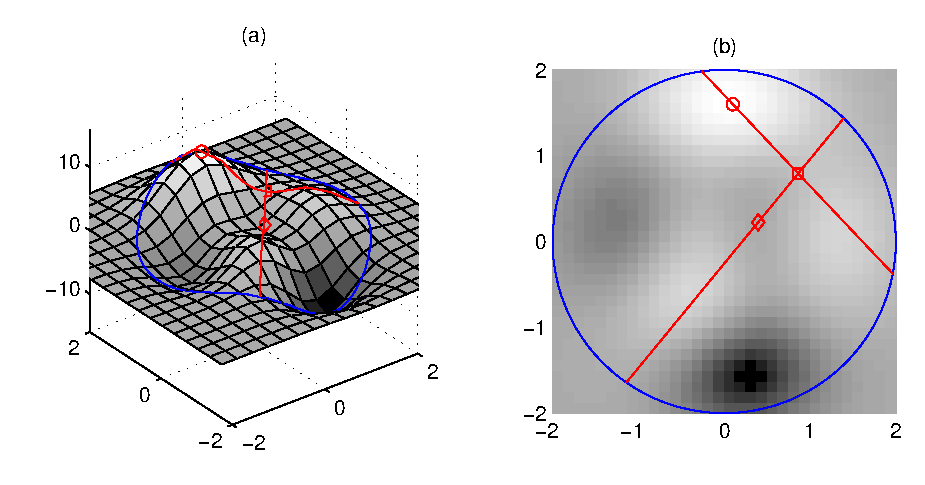
\includegraphics{figures/descent.epsg}
\caption{Schematic representation of gradient descent.  Points within the blue
circle are in \calF, the height of the surface the value of
(\ref{eqn:theory:cost function}) at that point.  (a) is a 3D view, (b)
is top view. Red lines show line searches; markers minimums.  Descent
from $\circ$ to $\Box$ to $\Diamond$, where it terminates due to
local minimum.}
\label{fig:gradient descent}
\end{center}
\end{figure}


\section{Normed boosting algorithms}

\section{Performance evaluation}


\subsection{Convergence of boosting}
Theorem: Given a weaklearner $\mathcal{L}$ and a training set $S$,
then either:
\begin{enumerate}
\item	The boosting algorithm will terminate; or
\item	There exists an iteration $t_{zero}$ such that for all $t \geq
	t_{zero}$ the training error $\epsilon_t = 0$.
\end{enumerate}
If for any training iteration $t$ we have $\epsilon_t > 1/2$ then the
boosting algorithm will terminate.  Assuming that this is not the
case, let us look at $\|b\|$.  As $t \rightarrow \infty$, $\|b\|
\rightarrow \infty$.  Thus, taking the normalised hypotheses $\bar{h}_i
= b_i \frac{h}{\sum b}$ we get the cost function as
\[
C(F_{t+1}) = \sum_{i=1}^{m} \exp\left\{ -y_i b_i h_i(x_i)
\right\}^{\|b\|}
\]
Now, we know from theorem (number?) that the boosting algorithm will
always find the global minimum of the cost function.  Since all $b_i >
0$, this is achieved when all training examples are classified
correctly...

Need a lot more work on this proof.  Do I want to show that since it
gets steeper and steeper, the cost of a negative sample gets too
large?  I don't think that the way I am doing it is going to work,
really.  I need to show that because
\begin{itemize}
\item	The weights for wrong samples are increasing exponentially,
	and
\item	The power that the cost function is raised to makes the wrong
	margin get worse and worse,
\end{itemize}
then the thingy gets minimised...

I need to bring the training error < 1/2 into it somewhere.  I think
that I can show that if
\begin{itemize}
\item	$\|b\|$ increases without bound; and
\item	$\epsilon_t$ is always < 1/2, then
\end{itemize}
I don't know!




\subsection{Size of $b$}
Theorem: The size of the $b$ weight vector, $\|b\| \rightarrow \infty$
as $t \rightarrow \infty$ (assuming the boosting algorithm doesn't
terminate).

Proof: ?


\subsection{Minimum margin}
Theorem: Given a particular learning algorithm $F$ and a training
set $S$, then define the minimum margin as
\[
m_{\min} = min_{\{x,y\} \in S} y_i F(x_i)
\]
Then the boosting algorithm will converge as $t \rightarrow \infty$ to
the solution which maximised the minimum margin.

Proof: For boosting we can write $F_t = b_1 f_1 + \cdots + b_t f_t$.
Then defining our \emph{normalised hypotheses} $\bar{f}_i$ as
\[
\bar{f} = \frac{b_i f_i}{\|b\|}
\]
such that $\hat{F}_t = \bar{f}_1 + \cdots + \bar{f}_t$, we can write
our cost function (reference?) as 
\[
C(b, S) = \sum_{i=1}^{m} \exp\{-y_i \bar{F}_t(x_i)\}^{\|b\|}
\]
We already know from the gradient descent theory (reference?) that we
are trying to minimise the cost function.  Now as $\|b\| \rightarrow
\infty$ (from the previous theorem) the largest value of $\exp\{-y_i
\bar{F}_t(x_i)\}$ will dominate, and so $C(b, S) \rightarrow exp\{\max
-y_i \bar{F}_t(x_i)\}$.  Thus, by minimising $C(b, S)$, we are making
$\min y_i \bar{F}_t(x_i)$ as large as possible; that is we are
maximising the minimum margin.


% pboosting.tex
% Jeremy Barnes, 22/9/1999
% $Id$

\chapter{$p$-boosting}

This chapter describes the concepts behind and a theoretical
justification of \emph{$p$-boosting}, a generalisation of the boosting
algorithm.  The treatment is somewhat abstract; further chapters will
be more concrete as practical issues are considered.

\section{Motivation: avoiding overfitting}



\subsection{Qualitative arguments}

Choo

\subsection{Quantitative arguments}
* By reducing covering numbers we get a better bound
* Thus use a $p$-convex hull instead of a $1$-convex hull
* Trade off: minimum margin may be reduced
* Thus, we would expect to see a curve (draw a graph, shaped like a parabola)
* Optimal $p$ value there, gives us the best error
* Draw a picture of the classes being smaller

\subsection{Summary}

\section{Generalisation performance of hypotheses in $\co_p(\calH)$}

Combining the covering-number generalisation performance bound
(\ref{eqn:covering number bound}) with the approximate values of
covering numbers for $p$-convex hulls (\ref{eqn:approx p-convex
bound}), we obtain the following theorem

\begin{theorem}[Approximate bound on generalisation performance]
The generalisation error of a hypothesis $F \in \co_p(\calH)$ where
$\calH$ has VC dimension???????? $d$ over a set of $m$ independent training
samples with probability at least $1 - \delta$ can be approximated by
%
\begin{equation}
R(F) \lesssim R_{\emp}^{\gamma}(F) + \sqrt{ \frac{8}{m} \left[ \log 2
+ c(p) \: d \: \left( \frac{2}{\gamma} \right)^{\frac{2p}{2-p}} \log
\left( \frac{2}{\gamma} \right) - \log \delta \right]}
\end{equation}
where $c(p)$ is a constant that depends upon $p$. 
%
\end{theorem}

This result is necessarily an approximation, due to the approximate
nature of the theorems it is based upon.

\section{Development of algorithms}

\subsection{Naive algorithm}

The naive algorithm (named with the benefit of hindsight) attempts to
modify the $b$ values of AdaBoost in a manner that will produce a
``$p$-convex like'' distribution of parameters on $p$.

The key feature of the algorithm is the calculation of the classifier
weights $b$.  Denoting the classifier weight that AdaBoost would have
used as $b'_t$, we use the formula
%
\begin{equation}
b_t = b'_t^\frac{1}{p} = \left[ - 1/2 \log \left( \frac{\epsilon_t}{1
- \epsilon_t} \right) \right]^\frac{1}{p}
\end{equation}
%
Thus, for $p < 1$ the hypotheses with low training error (and hence
high classifier weights) have these weights ``stretched'' out.  The
effect of $p$ is plotted figure \ref{fig:naive b values}.

\begin{linefigure}
\begin{center}
\includegraphics{figures/naive.epsg}
\end{center}
\begin{capt}{Effect of $p$ on classifier weights for naive algorithm}
The three lines show $b_t$ against $\epsilon_t$ for $p \in \{ 0.5,
0.7. 1.0 \}$.
\end{capt}
\label{fig:naive b values}
\end{linefigure}

There are two options for updating the sample weights $w$: based upon
the value of $b_t$, or based upon $b'_t$ (unchanged from AdaBoost).
The first option yields the equation
%
\begin{equation}
w_i|_{t+1} = \left\{
\begin{array}{cl}
	w_i|_t / Z_t \exp \left\{ b'_t^{1/p} \right\} & \qquad \qquad \mbox{if
	$f_t(x_i) = y_i$} \\
	w_i|_t / Z_t \exp \left\{ -b'_t^{1/p} \right\} 	& \qquad \qquad
	\mbox{otherwise} \\
\end{array} \right.
\end{equation}
%
The important point to notice is that the $1/p$ power (which is
greater than one for $p < 1$) is inside an exponential; this could
(and does) lead to the exponential function getting extremely large
(outside the limits of IEEE floating point numbers).  Thus we update
our sample weights based upon $b'_t$; they are identical to those
chosen by the boosting algorithm.

The naivity of the algorithm becomes apparent when considered in
the gradient descent framework.  As our sample weights are calculated
the same as AdaBoost; thus given an identical initial state both
algorithms would proceed in the same ``direction''.  However the step
sizes are different: AdaBoost performs a line search for the minimum
in this direction and moves to that point; whereas the naive algorithm
also searches for that point \emph{and then purposely avoids it!}
Experiments with this algorithm prove to have indifferent performance.

\subsection{Strict algorithm}

The strict algorithm is the purest of all $p$-boosting algorithms
considered in this thesis.  It performs gradient descent, using the
same cost function and inner product as AdaBoost, but uses the the
universal set $\calX = \co_p(\calH)$.  It is called the ``strict''
algorithm because it also performs its line searches along lines
$\ell$ where each point $p$ on $\ell$, $p \in \calX$.  In other words,
it confines its line search to the $p$-convex hull.  This idea is
illustrated in figure \ref{fig:strict line search}.

\begin{linefigure}
\begin{center}
\includegraphics{figures/strict_search.epsg}
\end{center}
\begin{capt}{Line search for strict $p$-boosting algorithm}
The strict $p$-boosting algorithm confines its line search to the
$p$-convex hull of points.
\end{capt}
\label{fig:strict line search}
\end{linefigure}

Algebraicaly, we are seeking a minimum of the expression
%
\begin{equation}
C(F_{t+1}) = \sum_{i=1}^{m} \exp \left\{ -y_i F_{t+1}(\bfx_i) \right\}
\end{equation}
%
subject to the constraint
Attempting to obtain a closed form solution for the minimum along this
line
 

\subsection{Sloppy algorithm}



\subsection{Gravity algorithm}

\subsection{Summary}

\section{Chapter summary}




% method.tex
% Jeremy Barnes, 22/9/1999
% $Id$

% Method baby...

\chapter{Experiments}
\label{chapter:method}

Extensive simulations of the $p$-boosting algorithms and AdaBoost were
run on a microcomputer in order to compare their performance, both
with the baseline AdaBoost algorithm, and with the theory developed in
previous chapters.  This chapter describes the experimental setup
(including a brief description of the software developed) and the
testing methodology to a level of detail sufficient to repeat the
experiments.

\section{Experimental setup}

In this section a summary of the equipment and computer software used
to perform the experiments is given.  The full source code, datasets
and test results are available on the CD-ROM attached inside the back
cover of this thesis.  Appendix \ref{appendix:cdrom} describes the
contents of this CD-ROM in more detail; appendix
\ref{appendix:datasets} the datasets; and appendix
\ref{appendix:software} the computer software.

\subsection{Hardware}

The simulations were run on three microcomputers.  The first was a
400MHz Celeron system with 256MB of memory, running RedHat Linux
version 6.0 and \MATLAB\ version 5.3.0.10183 (Release 11).  The second
was a 300MHz Celeron system with 128MB of memory, running RedHat Linux
version 5.2 and the same version of \MATLAB.  The third was a 233MHz
Cyrix M3 machine with 64MB of memory running Windows 95 version
4.00.1111 and \MATLAB\ version 5.0.0.4073 (Student version).

\subsection{Software}

Although an incidental part of the project, the software package that
was developed in order to perform the simulations is a significant
piece of work in its own right.  It was written from scratch to
allow an accessible and efficient entry into the project area--which
was not available at the commencement of the project.  In particular,
it includes many functions that allow visualisation of the algorithms.
Use of this package will significantly lower the difficulty of
beginning similar research or extending the ideas developed in this
project.

The software was written as a \MATLAB\ toolbox.  Two weak learning
algorithms (decision stumps and CART), several versions of the
Boosting algorithm (including all mentioned in this thesis), an
implementation of a Neural Network algorithm, an automated test
harness, and assorted analysis and visualisation functions are
included.  What follows is a brief description of the design and
implementation of the software package as a whole.  Individual
components are covered in appendix \ref{appendix:software}.

\subsection{Optimisation and numerical issues}

The code was profiled extensively using \MATLAB's inbuilt profiler,
and efficient algorithms selected for the frequently executed
sections.  Tight sections of code, and certain data and code
structures (for example, {\tt for} loops), which are inefficient under
\MATLAB, were recoded in \C\ to improve speed.  (Details of how
to interface this code were obtained from \cite{MathWorks96} and
\cite{MathWorks96a}.) As each function was optimised, its output was
compared with that of the un-optimised version to ensure equivalence
of the two versions of code.  The net effect of these optimisations
was that simulations which would have required several years to run as
initially coded were able to be run in a matter of days.

Minimising numerical errors was a major design goal.  Several sections
of code incorporate safeguards (such as periodic full recalculations
in loops that are optimised via incremental calculations) to minimise the
effect of numerical errors.  In addition, 64 bit IEEE double precision
floating point numbers are used exclusively.

In total, the source code was 270KB in size, comprising 235KB of
\MATLAB\ code and 35KB of \C\ code.  There are approximately 10000
lines in 191 \MATLAB\ {\tt .m} files and 1500 lines in 6 \C\ source
files.  All source code was maintained under the {\tt CVS} version
control system.

\section{Datasets}

A total of seven datasets were used in the experiments.  Four
(\ds{ring0}, \ds{ring10}, \ds{ring20} and \ds{ring30}) were
synthetic datasets, randomly generated from a known distribution with
noise added artificially.  Two other datasets (\ds{sonar} and
\ds{wpbc}%
\footnote{Wisconsin Prognostic Breast Cancer.}%
) were obtained from the UCI repository \cite{UCI}, and the
final dataset (\ds{acacia}) was ecological data used in a PhD thesis
\cite{Payne97}.  A summary of the features of each dataset appears in table
\ref{tbl:datasets} (Appendix \ref{appendix:datasets} describes the
datasets in more detail.)  This group was selected to cover a broad
range of situations:  the four \ds{ring} datasets allow the effect of
noise to be isolated and contain a very high sample-to-attribute
ratio;  the \ds{sonar} dataset is low-noise (generated from precise
measurements ) but contains a low sample-to-attribute ratio; and the
\ds{wpbc} and \ds{acacia} datasets are examples of difficult and very
difficult%
\footnote{Difficult and very difficult in that previous applications
of machine learning algorithms to these datasets produce indifferent
to poor results.}
real-world data.

\begin{table}
\begin{center}
\begin{tabular}{l c c r r r r}\hline
{\bf Dataset} & $\calI$ & $\calO$ & {\bf Artificial noise} & {\bf
Size} & {\bf Training samples} & {\bf Test samples} \\
\hline \hline
\ds{ring0} & $[0,1]^2$ & $\{\pm 1\}$ & 0\% & $\infty$ & 50 & 5000 \\
\ds{ring10} & $[0,1]^2$ & $\{\pm 1\}$ & 10\% & $\infty$ & 50 & 5000 \\
\ds{ring20} & $[0,1]^2$ & $\{\pm 1\}$ & 20\% & $\infty$ & 50 & 5000 \\
\ds{ring30} & $[0,1]^2$ & $\{\pm 1\}$ & 30\% & $\infty$ & 50 & 5000 \\
\hline
\ds{sonar} & $[0,1]^{60}$ & $\{\pm 1\}$ & 0\% & 208 & 70 & 138 \\
\ds{wpbc} & $\subset \bbR^{33}$ & $\{\pm 1\}$ & 0\% & 194 & 97 & 97 \\
\ds{acacia} & $\subset \bbR^{16}$ & $\{\pm 1\}$ & 0\% & 204 & 102 & 102 \\
\hline
\end{tabular}

{\small Note that samples with missing attribute values were excluded
from each dataset.}
\end{center}
\caption{Summary of dataset attributes}
\label{tbl:datasets}
\end{table}

\section{Testing}

In this section we detail the aims of the experiments, the procedure
that was followed, and how the results were summarised and analysed.

\subsection{Aims}
The aims of the experiments were four-fold:
%
\begin{enumerate}
\item	To test the generalisation performance of the $p$-boosting
	algorithms, and how this performance compares with the
	that of AdaBoost.  It was expected that the $p$-boosting
	algorithms would outperform AdaBoost on noisy datasets.

\item	To verify that the qualitative behaviour (and quantitative
	behaviour wherever possible) of the $p$-boosting algorithms
	matched the theory developed in chapters \ref{chapter:slt},
	\ref{chapter:boosting} and \ref{chapter:pboosting}:
	%	
	\begin{itemize}
	\item	The $p$ parameter controls the capacity of the
		function class.  Thus, a generalisation error vs $p$
		plot should have a minimum at some optimal value
		$p^{\ast}$ (figure \ref{fig:optimal p value}).
	\item	The confidence interval in theorem \ref{thm:p convex
		generalisation} decreases as $p \rightarrow 0$.  As a
		result, the true risk (test error) and empirical risk 
		(training error) curves should match closely as $p
		\rightarrow 0$.
	\end{itemize}
	
\item	To verify that the algorithms were operating as designed.
	It was expected that a distribution of classifier weights
	would show that most of the weight is given to fewer and fewer
	classifiers for low $p$ values.

\item	To test the efficiency of the algorithms as compared to
	AdaBoost.  An algorithm that generates a slightly better
	hypothesis but takes much longer to train may not be
	considered an improvement in some applications.
\end{enumerate}

\subsection{Method}

A total of 31 tests were run, as detailed in table
\ref{tbl:experiments}.  Each test involved training a particular
algorithm on a dataset (up to a maximum of \emph{Iterations} training
iterations).  The test was repeated for \emph{Trials} independent
trials, each time with a newly generated (\ds{ring*}) or randomly
permuted and partitioned (\ds{sonar}, \ds{wpbc}, \ds{acacia})
test and training dataset%
\footnote{Note that noise was added to the training \ds{ring*}
datasets but \emph{not} the test \ds{ring*} datasets.}%
, and this whole procedure repeated for each $p$ value.

\newcommand{\allp}{$\frac{1}{2} \leq p \leq 2; 10p \in \bbN$}
\newcommand{\lowp}{$\frac{1}{2} \leq p \leq 1; 10p \in \bbN$}
\begin{table}
\begin{center}
\begin{tabular}{r l l r r c}\hline
{\bf Number} & {\bf Algorithm} & {\bf Dataset} & {\bf Trials} &
{\bf Iterations} & {\bf $p$ values} \\
\hline\hline
1-4  & AdaBoost & \ds{ring*}   & 100 &  1000 & - \\
5    & AdaBoost & \ds{sonar}   &  30 &  1000 & - \\
6    & AdaBoost & \ds{wpbc}    &  50 & 10000 & - \\
7    & AdaBoost & \ds{acacia}  &  50 & 10000 & - \\
\hline
8-11 & Na\"{\i}ve & \ds{ring*} &  50 &  1000 & \allp \\
12   & Na\"{\i}ve & \ds{sonar} &  30 &  1000 & \allp \\
\hline
13-16 & Strict & \ds{ring*}    &  30 &  1000 & \allp \\
17    & Strict & \ds{sonar}    &  50 & 10000 & \allp \\
18    & Strict & \ds{wpbc}     &  20 &  5000 & \allp \\
19    & Strict & \ds{acacia}   &  20 & 10000 & \allp \\
\hline
21-24 & Sloppy & \ds{ring*}    &  30 &  1000 & \allp \\
25-28 & Sloppy & \ds{ring*}    &  30 & 10000 & \lowp \\
29    & Sloppy & \ds{sonar}    &  50 & 10000 & \allp \\
30    & Sloppy & \ds{wpbc}     &  20 &  5000 & \allp \\
31    & Sloppy & \ds{acacia}   &  20 & 10000 & \allp \\
\hline  
\end{tabular}

\small{The weak learning algorithm is always \emph{decision stumps}.}
\end{center}
\caption{Summary of experiments conducted}
\label{tbl:experiments}
\end{table}

The following data was recorded for each trial:
%
\begin{itemize}
\item	All test parameters;
\item	Test and training datasets;
\item	Training and test error (unweighted) at each iteration;
\item	Margins of the training samples at both the iteration with the
	minimum \emph{test} error and the final iteration;
\item	Classifier weights at the final iteration.
\end{itemize}


\subsection{Analysis}

More than two gigabytes of data was generated in the course of
testing.  This data was summarised across all trials for each (test,
p-value) combination, and a summary file created.  The summary file
contained the following information:
%
\begin{itemize}
\item	The mean and standard deviation of test and training error
	curves at each iteration;
\item	The number of trials that had not aborted before each
	iteration (recall that the algorithms would abort if the
	training error exceeded $\frac{1}{2}$, fell below $0$, or if
	the cost function was strictly increasing); 
\item	The value of the best (lowest) test error for each trial, and
	the number of training iterations after which this best error
	value occurred;
\end{itemize}
%
Each of the $p$-boosting algorithms had further statistics produced
for each $p$ value.  These statistics were:
%
\begin{itemize}
\item	The mean and standard deviation of the best test error at each
	$p$ value, over all trials;
\item	The mean and standard deviation of the number of training
	iterations the best error was produced at, over all trials.
\end{itemize}

For each of the $p$-boosting algorithms, a crude form of structural
risk minimisation (see section \ref{sec:theoretical overfitting}) was
then performed, by selecting the $p$ value with the \emph{lowest mean
best test error} to be $p^{\ast}$ (see figure \ref{fig:effect of p} on
page \pageref{fig:effect of p}).  This is the $p$ value that is used 
whenever comparisons of the performance of algorithms are made (it
makes little sense to compare anything but the \emph{best}
performance!)  The entire analysis described above was repeated for
each dataset.






% results.tex
% Jeremy Barnes, 22/9/1999
% $Id$

\chapter{Results and discussion}
\label{chapter:results}

This chapter summarises the outcome of the experiments described in
chapter \ref{chapter:method}, discusses their features, and compares
them with the results expected from the theory in chapters
\ref{chapter:slt} to \ref{chapter:pboosting}.

An opening observation is that Boosting algorithms are very erratic in
their behaviour.  As a result, it is difficult to make conclusive
judgments based on individual observations; at the very least
statistical measures need to be used, and even so a huge amount of
computing resources are required to obtain sufficient results to make
confident conclusions.

\section{Generalisation performance}

Figure \ref{fig:test err summary} is a high-level summary of results
on the generalisation performance of the $p$-boosting variants as
compared to AdaBoost.  The graph compares the result from the
hypothesis chosen via SRM (section \ref{sec:theoretical overfitting})
with AdaBoost. 

It can be seen that although the average generalisation performance of
the $p$-boosting algorithms is in most cases slightly better than that
of AdaBoost, only in a few cases is the difference significant.  The
only dataset upon which the strict algorithm generalises significantly
better than AdaBoost is \ds{acacia}.  The sloppy algorithm generalises
significantly better on \ds{ring10}, \ds{ring20}, \ds{ring30} and
\ds{acacia}; while the na\"{\i}ve algorithm always outperforms
AdaBoost by a small (never statistically significant) amount.

Thus, the sloppy algorithm appears to outperform AdaBoost on the noisy
datasets considered (recall that the \ds{acacia} dataset was chosen as
it was a difficult dataset).  This behaviour was expected--the
algorithm was specifically designed to implement capacity control.  It
also appears that the na\"{\i}ve algorithm has little effect on
generalisation performance (a somewhat surprising result--the
discussion in chapter \ref{chapter:pboosting} concluded that the
algorithm should be \emph{worse} than AdaBoost.  We shall return to
this result shortly).


\begin{linefigure}
\begin{center}
\includegraphics{figures/test_err_summary.epsg}
\end{center}
\begin{capt}{Comparison of AdaBoost and $p$-boosting test generalisation
performance}{fig:test err summary}
The diagonal line indicates points where the test error of AdaBoost
and the $p$-boosting algorithm are equal.  Points above line indicate
that the $p$-boosting algorithm generalises better than AdaBoost.  The
light bars indicate the spread of the trials, and are one standard
deviation in length either side of the mean.

\noindent{\bf Key:} $\bullet$ \ds{ring0}, $\times$ \ds{ring10}, $\circ$
\ds{ring20}, $\ast$ \ds{ring30}, $\Box$ \ds{sonar}, $\bigtriangleup$
\ds{wpbc}, $\Diamond$ \ds{acacia}.
\end{capt}
\end{linefigure}


\section{Training time}

Figure \ref{fig:test iter summary} details how the training times of
$p$-boosting algorithms compare with AdaBoost.  It is quite clear that
the sloppy and strict algorithms require slightly to substantially
more training iterations than AdaBoost.  Thus, the improved
generalisation performance of these algorithms comes at the cost of
increased training time.  In section \ref{sec:training curves} we will
examine the mechanisms that cause the increased training time, and
suggest remedies.

\begin{linefigure}
\begin{center}
\includegraphics{figures/test_iter_summary.epsg}
\end{center}
\begin{capt}{Comparison of AdaBoost and $p$-boosting training
times}{fig:test iter summary} 
Both axes measure numbers of iterations.  The $y$ axis measures the
average number of iterations required for AdaBoost to reach the
minimum of the test error; the $y$ axis is the same statistic for the
$p$-boosting variant (at $p^{\ast}$).  Points above the line indicate
that AdaBoost requires more iterations to train than the $p$-boosting
algorithm.  Uneven error bars are due to the logarithmetic scale.
Marker symbols indicate datasets: 

\noindent{\bf Key:} $\bullet$ \ds{ring0}, $\times$ \ds{ring10}, $\circ$
\ds{ring20}, $\ast$ \ds{ring30}, $\Box$ \ds{sonar}, $\bigtriangleup$
\ds{wpbc}, $\Diamond$ \ds{acacia}.
\end{capt}
\end{linefigure}


\section{Effect of $p$ value on generalisation performance}

Figure \ref{fig:effect of p} expands the information in figure
\ref{fig:test err summary} to include information on \emph{all} values
of $p$ (not just the best value $p^{\ast}$).

Consider first the sloppy algorithm (dashed line in figure
\ref{fig:test err summary}).  When trained on the noisy \ds{ring}
datasets, this algorithm appears to be implementing capacity control
as expected, with the generalisation error reaching a minimum at an
optimal value of $p$ (compare with figure \ref{fig:optimal p value} on
page \pageref{fig:optimal p value}).  It is difficult to pinpoint
exactly where this $p^{\ast}$ value is due to the coarse resolution
along the $p$ scale, but it appears that $0.8 \leq p^{\ast} \leq 1.2$.

The results on other datasets are less clear: the low-noise datasets
\ds{ring0} and \ds{sonar} show a flat curve with no obvious minima
(the slight downward slope indicating that such a minima may exist for
$p > 2$); whereas the curves for \ds{wpbc} and \ds{acacia} both appear
to be almost random.

The performance of the strict algorithm is very poor for $p < 1$ (due
to the algorithm terminating training after few iterations); for $1
\leq p < 2$ it appears to reach a reasonable hypothesis (and a
particularly good one in the case of the \ds{wpbc} and \ds{acacia}
datasets).  It shares the sloppy algorithm's general down-sloping
characteristic on low-noise datasets, and also appears to reach a
minimum on the higher noise datasets.  It is interesting to note that
the $p^{\ast}$ value differs substantially between the strict and
sloppy algorithms.  This is a counter-intuitive result: the optimal
capacity should be an intrinsic property of the \emph{dataset}, not
the algorithm, when both algorithms are operating from the same
hypothesis class $\calX = \co_p(\calH)$.

The performance of the na\"{\i}ve algorithm does not deviate
significantly from that of AdaBoost.  The $p$ parameter appears to
have little effect on this algorithm.

In summary, it appears that the strict and sloppy algorithms match the
expected behaviour of an optimal $p$ value minimising test error for
the noisy datasets, but not for low-noise datasets (although there is
an indication that maybe $p^{\ast} > 2$, and thus is off the scale of
figure \ref{fig:effect of p}).

\begin{linefigure}
\begin{center}
\hspace*{-1cm}\includegraphics{figures/effect_of_p.epsg}
\end{center}
\begin{capt}{Effect of $p$ on generalisation error}{fig:effect of p}
Average test error of each algorithm over all trials: AdaBoost (thick
line), strict (thin solid), sloppy (dash-dot) and na\"{\i}ve (dotted)
is shown for each dataset.  The bullets $\bullet$ indicate the value
$p^{\ast}$ which is used in figure \ref{fig:test err summary}.  Note
that the sloppy algorithm was not trained on the \ds{wpbc} or
\ds{acacia} datasets.  The $y$ (test error) scale varies.
\end{capt}
\end{linefigure}

\section{Training curves}
\label{sec:training curves}

Figure \ref{fig:training curves} shows a selection of training curves
from the strict and sloppy algorithms, all training on the \ds{ring30}
dataset.  There are three interesting observations concerning these
curves.  Firstly, part (a) shows that the training error for the
strict algorithm, $p=0.5$ is actually \emph{increasing} with the number
of iterations!  This behaviour often recurs immediately before
training is aborted.  Thus, there is an indication of instability of
the strict and decision stumps combination; the mechanism behind it is
unclear and was not investigated further.

Secondly, for $p=0.5$ (parts (a) and (d)), the test error and training
error curves follow each other quite closely.  This behaviour has a
theoretical explanation: for low values of $p$, the covering numbers
of $\co_p(\calH)$ (and thus the confidence interval of figure
\ref{fig:boosting generalisation bound form}) are small.  We would
therefore expect the test and training curves to match closely--which
they do.

The third observation concerns the training of the sloppy algorithm.
For $p \in \{0.5, 1\}$ the behaviour is quite erratic on a fine scale,
but steady on average (random oscillations about a steady average
value).  It appears that this algorithm is ``thrashing around'' in the
cost space, unable to find a direction (hypothesis) which will
significantly reduce the cost functional.  We will see shortly that
the algorithm eventually will converge; the $10^3$ iterations were not
sufficient for this to happen.  As a result, the results for the
sloppy algorithm may be somewhat skewed towards higher test error
values.

\begin{linefigure}
\begin{center}
\includegraphics{figures/training_curves_strict.epsg}
\includegraphics{figures/training_curves_sloppy.epsg}
\end{center}
\begin{capt}{Selected test/training error curves}{fig:training curves}
The curves show training error (grey line) and test error (black
line) against iteration number.  Each point of both curves is
averaged over all trials that had not aborted at the specified
iteration number.
\end{capt}
\end{linefigure}

Figure \ref{fig:weight distribution} is a more detailed look at the
mechanics of the training process for the AdaBoost algorithm (as a
reference) and the strict and sloppy algorithms.

\begin{linefigure}
\begin{center}
\hspace*{-1cm}\includegraphics{figures/weight_distributions.epsg}
\end{center}
\begin{capt}{Details of the training process}{fig:weight distribution}
The above graphs detail a \emph{single} training run (not average
behaviour).  All three algorithms were trained to 10000 iterations,
using the \ds{ring30} distribution, for $p=1$ (black), $p=0.5$
(dark gray) and $p=1.5$ (light grey).  Parts (a) to (c) show
classifier weights; parts (d) through (f) are the corresponding
training error curves.  Note that (c) contains the \emph{same} data
plotted on two different scales--the two steep curves belong to the
right hand scale.  (Note log scale on classifier weight graph).
\end{capt}
\end{linefigure}

We first describe the behaviour of AdaBoost, to provide a basis for
comparison with the other algorithms.  Part (a) shows that the
classifier weights of the AdaBoost algorithm decrease as a constant
power of $t$ (note the logarithmetic scale)%
\footnote{A straight line on a log-log plot indicates a relationship
of the form $y = x^{\kappa}$, where $\kappa$ is the slope of the line.}
until training error reaches zero, and then oscillate about this same
value.  Thus, the early weights are slightly larger than the later
weights, but all are of a significant size.

Contrast this behaviour with that of the strict algorithm in part (b).
Considering the $p=1$ curve in part (b)%
\footnote{The $p=0.5$ curve aborted training after 2 iterations.}
it is clear than these weights continue decreasing as $b_t =
t^{-\lambda}$.  The nearly flat training error curve is thus explained
by the classifier weights getting too small for the weak hypotheses
$h_t$ as $t$ increases to have any effect on the combined hypothesis
$H_t$.  The $p=1.5$ curve in part (b) matches the shape of the
AdaBoost curve until approximately 2000 iterations, where the weights
also begin to drop off.  The magnitude of the weights in the flat
section are however much smaller than those of AdaBoost; it may be a
consequence of this fact that the strict algorithm takes about 10
times longer to converge than AdaBoost. 

Part (c) contains some very interesting behaviour which goes some way
towards explaining the noisy part of the training error curve.  Noting
that the scale on the $y$ axis reaches $10^{-300}$, it is clear that
most of the classifier weights are so small as to be practically
zero.  The second obvious feature is the ``kink'' in the $p=1$ and
$p=0.5$ curves at approximately 800 iterations; this kink corresponds
to the end of the noisy sections of part (f) and a (comparatively)
rapid decrease in training error.  The magnified curves on the right
of part (c) (where we see the iterations with high weights for $p \in
\{1, 1.5\}$) show that only a few hypotheses $h_t$ have significant
weight in $H_t$, as designed.

In summary, these results indicate that the \emph{concept} of using a
$p$-convex hull is a good one: we saw in figure \ref{fig:test err
summary} that the final hypotheses generated by the sloppy algorithm
often generalise better than AdaBoost, and figure \ref{fig:weight
distribution} shows that this final hypothesis is indeed sparse in
its parameter weights.  The problem is in the \emph{implementation}:
a very large number of iterations are required to generate this sparse
hypothesis; when the weights of hypotheses generated by most
iterations are several \emph{hundred} orders of magnitude below being
significant.


\subsection{Remedies for inefficient training}

These observations would suggest that the starting point for the
gradient descent algorithm is particularly bad; as a result a lot of
iterations are wasted in getting to a good starting point (the kink in
part (c)) from where the optimisation can converge quite quickly.
Another optimisation strategy that is less sensitive to starting point
may prove to be more efficient (such as annealing); this algorithm
could prove to be \emph{very} useful if the slow initial training
could be avoided.

Of course, it is not at all clear how to ``start at a different
point'', as the algorithms as currently implemented start in a
$1$-dimensional space and add one dimension per iteration.

Alternatively, it may be possible to accelerate the training of the
sloppy algorithm by choosing a more aggressive cost function.  For
example, the cost function
%
\begin{equation}
c(\alpha) = e^{-\alpha t^\lambda}
\end{equation}
%
where $t$ is the iteration number, and $\lambda>0$ a constant
parameter would serve to accelerate training, where $\lambda$ controls
the degree of acceleration ($\lambda=0$ is equivalent to the sloppy 
algorithm).  The main feature of this cost function is that it gets
steeper as the number of iterations increases, and thus has the
property of guaranteed zero training error.  However, it may be that
this algorithm would have its own problems.  Insufficient time was
available to perform experiments.

\section{Further observations}

The following discussion concerns noteworthy features that were
observed but have not been described previously.

\subsection{Hard datasets}

The full set of training curves in appendix \ref{appendix:allgraphs}
show that very rarely were the learning machines considered here
(including AdaBoost) able to train for more than about 100 iterations
on the \ds{acacia} dataset.  In the case of AdaBoost and the strict
algorithm, the weak learner was not sufficiently good to continue
generating hypotheses with a training error of less than
$\frac{1}{2}$.

The \ds{wpbc} dataset was also difficult, with only about one half of
the trials making it through 1000 training iterations without
terminating.  A stronger weak learning algorithm (such as a deeper
decision tree), or a method of restarting training after it has
aborted (one such is described in \cite{Bauer99}) could be used to 
avoid termination of the algorithm.  In contrast, only the strict
algorithm terminated on any other datasets.

\subsection{Na\"{\i}ve $p$-boost}

Observation of figures \ref{fig:test err summary} and \ref{fig:effect
of p} show that the performance of the na\"{\i}ve algorithm closely
matches that of the AdaBoost algorithm; the variation between the two
being insignificant (the two algorithms are equivalent when $p = 1$.
This is a surprising result--in chapter \ref{chapter:pboosting} it was
shown that the na\"{\i}ve algorithm systematically chooses a
\emph{less than optimal solution} by modifying distance chosen by the
line search.

Thus, we observe that AdaBoost is quite robust to modifications to the
\emph{classifier} weights (of course, these modifications were in the
specific form of a monotonic transform--arbitrary modifications would
likely have an adverse effect).  It would be expected, therefore, that
the \emph{sample} weights must cause the success of the algorithm.
This assertion was also made by Breiman:

\begin{quotation}
After testing [an algorithm equivalent to AdaBoost] I suspected that
its success lay not in its specific form but in its adaptive
resampling property, where increasing weight was placed on those cases
more frequently misclassified.  \cite{Breiman96}
\end{quotation}



% conclusion.tex
% Jeremy Barnes, 6/10/1999
% $Id$

\chapter{Conclusion}
\label{chapter:conclusion}

This thesis has considered variants of the AdaBoost machine learning
algorithm, with the desirable property of explicit capacity control,
implemented by confining the combined hypotheses to a $p$-convex hull
of underlying hypotheses.  Theoretical results indicate that these
algorithms should outperform AdaBoost on noisy datasets.

Several ``$p$-boosting'' algorithms were developed: a na\"{\i}ve
approach (which showed no noticeable improvement over AdaBoost), a
``strict'' algorithm confined strictly to the $p$-convex hull at all
times, and a ``sloppy'' variant less restricted during the line
search.

The strict algorithm showed a small improvement over AdaBoost over the
difficult \ds{acacia} dataset, but in general performed poorly
(particularly for $p < 1$).  The poor performance was caused by the
cost functional proving to be strictly increasing, or to have a
minimum very close to the previous hypothesis (in effect the gradient
descent algorithm did not move significantly from its starting point).
Analysis of the features of the cost functional showed that ``easy''
samples produced hill-shaped sample cost functions that would
contribute to a strictly a increasing cost functional.

The sloppy algorithm performed well on noisy datasets, with the shape
of the capacity-vs-gener\-alis\-ation error curve matching the theoretical
prediction, and the generalisation error at the optimal
$p$ value significantly (up to 25\%) improved on AdaBoost (which
already performs \emph{very} well).  While it appears that this
algorithm did find a good solution, which was sparse as predicted by
the theory, it did so in a very inefficient manner (particularly for
$p < 1.2$), with up to several thousand iterations spent adding
hypotheses with weights several hundred orders of magnitude below a
significant level.  A form of the cost function designed to
accelerate the training process is proposed as a potential solution;
alternatively a different optimisation strategy could be used.

It can be concluded that the \emph{concept} of using a $p$-convex hull
has merit as a method of increasing the noise-tolerance of the already
very strong AdaBoost algorithm, but the algorithms that were developed
to \emph{implement} the idea were lacking.

No quantitative comparisons between $p$-boosting algorithms and
other AdaBoost derivatives with similar goals (soft margins
\cite{Ratsch98}, DOOM I/II \cite{Mason99, Mason99a}) were made.
However, these approaches do not appear incompatible with the $p$-convex
hull approach; it is likely that a combined approach would be superior
to both.



\appendix

% Put it back to normal for the non-body parts of the thesis.
\renewcommand{\baselinestretch}{1.0}
% Execute a change in font size to make it happen
\small\normalsize

% stumps.tex
% Jeremy Barnes, 22/9/1999
% $Id$

\chapter{Decision Stumps}
\label{chapter:stumps}

We digress slightly from the theory to look at a simple example of a
practical learning machine, that has some nice properties (and was used
to perform all of the experiments in this thesis).
The \emph{decision stumps} algorithm is a very simple learning
machine.  As a stand-alone tool it is almost useless; but when
combined with the boosting algorithm it can generate very good
hypotheses.  Additionally, it has a fixed VC dimension which aids in
the analysis of learning algorithms based upon it.

\section{The decision stump learning machine}

The decision stump algorithm divides the input space into two disjoint
regions, with the boundary between them running perpendicular to one
of the axes (the decision boundary is an axis-orthogonal hyperplane).
Each region is given a label.  Figure \ref{fig:decision stump} shows
the decision boundaries of two decision stump classifiers.

\begin{linefigure}
\begin{center}
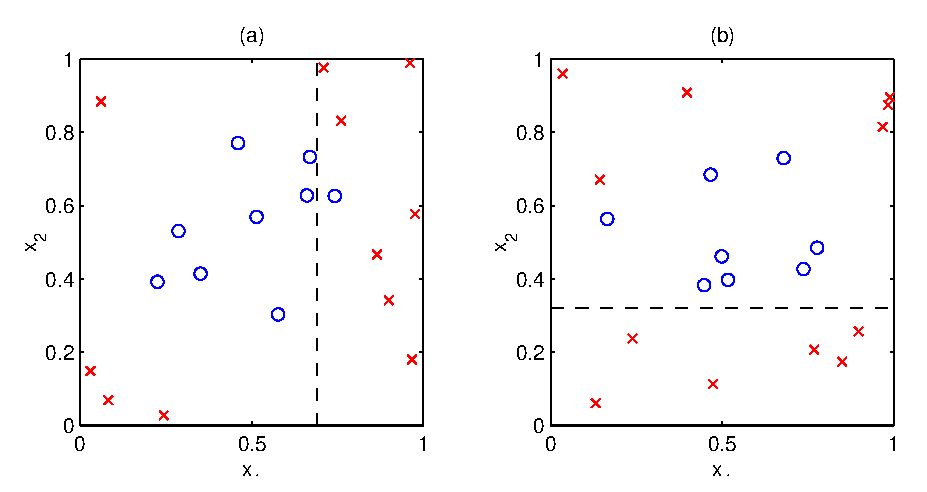
\includegraphics{figures/stumpdiagram.epsg}
\end{center}
\begin{capt}{A decision stump classifier}{fig:decision stump}
Part (a) shows the decision boundary of a decision stump classifier,
and the label of each region.  Part (b) the data it was trained on,
where $\times = -1$ and $\circ = +1$.
\end{capt}
\end{linefigure}

The algorithm constructs a list of possible split locations and
exhaustively searches this list for the minimum of the cost function
(misclassification risk).  Possible split locations are determined by
projecting every data point onto each axis in turn, and bisecting each
pair of consecutive projections to determine the candidate point.
Figure \ref{fig:candidate points} illustrates the process.

\begin{linefigure}
\begin{center}
\includegraphics{figures/stumpcandidates.epsg}
\end{center}
\begin{capt}{Candidate points for decision stump split}{fig:candidate points}
Data points ($\times$) are projected onto the axes.  Each consecutive
pair of projections is then bisected, to generate candidate split
points ($\bullet$).
\end{capt}
\end{linefigure}

\section{Properties of decision stumps}

\begin{theorem}[VC dimension of decision stumps]
\label{theorem:vcdim stumps}
The set $\mathcal{S}$ of decision stump classifiers on an domain
$\calI \subseteq \bbR^d$ has a VC dimension of bounded by 
%
\begin{equation}
\VCdim(\calS) \leq d + 1
\end{equation}
%
and, for a training set $X$ of size $m \gg d$ with sufficient
variation in its $\bfx$ parameters, has a constant VC dimension.
%
\end{theorem}

\proof The set $\calS$ of all axis orthogonal hyperplanes
is contained within the set $\calH$ of $d$ dimensional hyperplanes
(which has VC dimension $d+1$.

That the VC dimension is constant is intuitively sensible
but tricky to prove formally.  As no subsequent result \emph{relies}
upon this property, we will not elaborate further.

% newton-raphson.tex
% Jeremy Barnes, 16/10/1999
% $Id$

\chapter{Details of Newton-Raphson method}
\label{appendix:newton-raphson}

This appendix details Newton-Raphson search implemented in the sloppy
and strict algorithms.

The following code sequence, which is edited to remove debugging code,
is obtained from the file {\tt trainagain.m} in the {\tt normboost}
object folder.

\begin{verbatim}
function [obj_r, context] = trainagain(obj)

if (aborted(obj))
   obj_r = obj;
   warning('trainagain: attempt to train when training aborted');
   return;
end

x_data = x(obj);  y_data = y(obj);  w_data = w(obj);  p = norm(obj);

% create and train a new classifier
new_c = train(weaklearner(obj), x_data, y_data, w_data);

% find the training error
new_error = training_error(new_c);

% see what this algorithm does to our data
new_y = classify(new_c, x_data);


% find if we need to abort
if (new_error == 0)
   % Zero error -- one classifier can do perfectly by itself
   obj_r = abort(obj);
   return;
end

if (new_error >= 0.5)
   % Error of 0.5 -- random guessing does just as well
   obj_r = abort(obj);
   return;
end

% Calculate alpha
if (iterations(obj) == 0)
   % First iteration -- set alpha to 1 and marg to the margins of the
   % trained weak learner.

   alpha = 1.0;
   marg = (y_data*2-1) .* (new_y*2-1);
   new_b = [1.0];

else
   % Calculate alpha using a line search.  This uses the Newton-Raphson method
   % to find the minimum.

   % Initialisation
   new_alpha = 0.5 / iterations(obj);
   d = 1;
   min_d = inf;
   max_d = -inf;
   last_c = 1000000;
   tolerance = 0.001;
   
   
   % Iterate
   iter = 0;
   while ((abs(d) >= tolerance) & (iter < 1000))
      alpha = new_alpha;
      
      [c, d, d2] = eval_cf(obj, new_c, alpha);
      min_d = min([d min_d]);
      max_d = max([d max_d]);
      
      % Handle d2=0 in a very crude manner, which allows us to continue
      if (d2 < eps)
	 d2 = 0.01;
      end
      
      new_alpha = alpha - (d / d2);
      
      % Never let alpha move more than half the distance to zero.  This
      % can lead to alpha < zero, which causes all kinds of problems.
      min_alpha = alpha / 2;
      new_alpha = max([min_alpha new_alpha]);
      
      % This stopping rule is designed to detect the situation where there
      % is no solution as dc/dalpha > 0 for all alpha.  It halts the
      % training if there is no change in the cost function, and we have
      % not found a zero crossing of the derivative.
      if ((abs(c - last_c) < tolerance) & (min_d*max_d > 0))
	 break;
      end
      last_c = c;
      
      iter = iter + 1;
   end

   % Test for lack of convergence
   if (iter >= 100)
      warning('trainagain: failed to converge after 100 iterations');
   end
   
   % Test for minimum/maximum at our found point.  We do this on the sign
   % of the second derivative: if positive, we found a minimum; if
   % negative we found a maximum.
   [c, d, d2, marg] = eval_cf(obj, new_c, alpha);
   
   if (d2 <= 0.0)
      alpha = 0;
      obj = abort(obj);
   end
   
   % Calculate our new classifier weights   
   old_b = classifier_weights(obj);
   new_b = [old_b alpha] ./ pnorm([old_b alpha], p);

   one_norm = pnorm(new_b, 1)
end

% Update the sample weights.  These are calculated as the derivatives
% of the cost _function_ (not functional) and then normalised with a
% 1-norm equal to 1.
%
% For a cost function of exp(-x), dc/dx = -exp(-x).  The minus gets
% normalised out, and can be ignored.

new_w = exp(-marg);
new_w = new_w ./ sum(new_w);


% Update our weights
obj = add_iteration(obj, new_c, new_b, new_w);
obj.margins = marg;

obj_r = obj;
\end{verbatim}

% datasets.tex
% Jeremy Barnes, 16/10/1999
% $Id$

\chapter{Description of datasets used}
\label{appendix:datasets}

We include a description of the datasets.

\section{Ring dataset}

\section{Acacia dataset}

\section{Sonar dataset}

\section{Wisconsin prognostic breast cancer dataset}


% cdrom.tex
% Jeremy Barnes, 16/10/1999
% $Id$

\chapter{Contents of the attached CD-ROM disk}
\label{appendix:cdrom}

The attached disk is a standard 650MB cd-recordable that should be
readable in any CD-ROM player.  It contains a Microsoft Joliet file
system, readable by the Windows 95 and Linux%
\footnote{With the appropriate kernel options installed.}
operating systems.


% software.tex
% Jeremy Barnes, 22/10/1999
% $Id$

% This file briefly describes the computer software that I developed for
% this project, and provides some examples of its use.

\chapter{Software}
\label{appendix:software}

\section{Introduction}

\section{Installation}

\section{Classes and functions}

\subsection{Dataset}
The {\tt dataset} class encapsulates a dataset with several input
attributes and one output 

\begin{tabular}{ll}
\hline
dataset 	& Create a dataset object \\
\hline
numcategories 	& Return number of categories (binary=2)\\
numsamples 	& Return number of samples \\
dimensions	& Return number of dimensions (attributes) \\
\hline
data		& Return samples and labels \\
x\_values	& Return samples \\
y\_values	& Return labels \\
\hline
datagen		& Generate data from a distribution \\
load		& Load a dataset \\
addsamples	& Add data to the dataset \\
\hline
partition	& Split dataset into two parts \\
randomize	& Randomly permute the order samples \\
\hline
dataplot	& Generate a plot of the dataset \\
\hline
\end{tabular}

\subsection{Classifier}

The classifier type is the ancestor of all of the learning machines.
The following functions apply to both the classifier type and all of
its descendent types.

\begin{tabular}{ll}
\hline
classifier		& Create a classifier object \\
\hline	
dimensions		& Return dimensions of input space \\		
numcategories		& Return number of categories \\
\hline
train			& Train a classifier \\
classify		& Classify a set of samples \\
empirical\_risk		& Return the empirical risk over a dataset \\
margins			& Return the margins of a set of samples \\
\hline
trained\_samples		& Return the samples trained over \\
training\_error		& Return the empirical risk over training dataset \\
\hline
marginplot		& Plot margins of a dataset \\
plot\_classification	& Plot how samples get classified \\
plot\_decision\_boundary	& Approximate and plot decision boundary from margins \\
\hline
\end{tabular}{ll}


\subsection{CART}

The CART classifier is a full decision-tree based algorithm (a
generalisation of Decision Stumps).  In addition to the functions
inherited from classifier, it includes the following functions.

\begin{tabular}{ll}
\hline
cart			& Create a CART classifier \\
\hline
classify		& Classify some data \\
classification\_error	& Return error of previous classify operation \\
\hline
train			& Train CART classifier \\
training\_error		& Return empirical risk over training dataset \\
\hline
plotboundary		& Equivalent to plot\_decision\_boundary \\
plottree		& Divide plane into coloured areas \\
printtree		& Print textual representation of tree \\
treesize		& Return number of leaf nodes in tree \\
\hline
\end{tabular}

\subsection{Decision stump}

\begin{tabular}{ll}
\hline
decision\_stump		& Create a decision stump classifier \\
\hline
margins			& Return margins \\
marginplot		& Plot margins \\
\hline
plottree		& Graphical representation of decision tree \\
printtree		& Textual representation of decision tree \\
treesize		& Return number of leaf nodes (always 2) \\
\hline
\end{tabular}

\subsection{Neural network}

\begin{tabular}{ll}
\hline
neural\_net		& \\
\hline
classify		& \\
\hline
train			& \\
trainagain		& \\
trainfirst		& \\
training\_data		& \\
training\_error		& \\
training\_labels	& \\
training\_samples	& \\
\hline
test			& \\
\hline
get			& \\
set			& \\
\hline
hidden\_units		& \\
learning\_rate		& \\
momentum		& \\
\hline
hidden\_weights		& \\
output\_weights		& \\
iterations		& \\
\hline
\end{tabular}

\subsection{Boost}

abort
aborted
add\_iteration
as\_boost
as\_classifier
boost
classifier\_weights
classify
iterations
margins
sample\_weights
test
train
trainagain
trained\_samples
trainfirst
training\_error
update\_margins
w
weaklearner
weight\_density\_plot
wl\_instance
x
y

\subsection{Strict $p$-boosting algorithm}

eval\_cf
norm
normboost
trainagain
update\_margins

\subsection{Sloppy $p$-boosting algorithm}

eval\_cf
normboost2
trainagain
update\_margins

\subsection{Na\"{\i}ve $p$-boosting algorithm}

as\_boost
b\_plot
boost
cvs
disp
disp\_info
get\_p
p\_boost
trainagain


\subsection{Visualisation functions}

density\_plot
load\_pgm
plot\_domain
plot\_margin\_distribution
plot\_region
twoclass\_colormap
twoclass\_density\_to\_color
uniform\_color\_cube


\section{Testing and experiments}

\begin{tabular}{ll}
\hline
maketest		& \\
\hline
runtest			& \\
\hline
summarise		& \\
summarise\_boost	& \\
meta\_summarise		& \\
\hline
get\_test\_info		& \\
get\_test\_results	& \\
\hline
display\_meta\_summary	& \\
display\_results	& \\
plot\_results		& \\
\hline
\end{tabular}
% allgraphs.tex
% Jeremy Barnes, 22/10/1999
% $Id$

% This file provides about 10 million graphs which cover pretty much all
% the information.

\newcommand{\ig}[1]{\hspace*{-1cm}\includegraphics{graphs/#1}}

\chapter{Detailed results}
\label{appendix:allgraphs}

This appendix includes all test/training curves, and scatterplots of
the best test error against $p$, and the best test iteration against
$p$.  Axis labels are neglected in order to avoid clutter.

The training curves are averages over all trials.  The $x$ axis is
trial number; the $y$ axis is test or training error.  Test error is
the black curve; training error is the grey curve.  The number of
trials completing a certain number of iterations is plotted in the
dashed line, on the right hand scale.

The best test error and best test iteration curves show the scatter
over all trials.  The $x$ axis is the $p$ value; the $y$ axis the best
test error or number of iterations at which this occurs.

The thin lines indicate averages (these are also plotted in figure
\ref{fig:effect of p}).  The dotted line indicates one standard
deviation above and below.  The thick line indicates AdaBoost's result
over that training set, with the thick dotted line one standard
deviation above and below.

\section{AdaBoost}

\ig{boost-summary}

\section{Strict}

\subsection*{Best test error vs $p$}

\ig{strict-err-summary}

\subsection*{Best test iter vs $p$}

\ig{strict-iter-summary}

\subsection*{Training curves}

\subsubsection*{\ds{ring0}}\ig{strict-ring0}
\subsubsection*{\ds{ring10}}\ig{strict-ring10}
\subsubsection*{\ds{ring20}}\ig{strict-ring20}
\subsubsection*{\ds{ring30}}\ig{strict-ring30}
\subsubsection*{\ds{sonar}}\ig{strict-sonar}
\subsubsection*{\ds{wpbc}}\ig{strict-wpbc}
\subsubsection*{\ds{acacia}}\ig{strict-acacia}



\section{Sloppy}

\subsection*{Best test error vs $p$}

\ig{sloppy-err-summary}

\subsection*{Best test iter vs $p$}

\ig{sloppy-iter-summary}

\subsection*{Training curves}

\subsubsection*{\ds{ring0}}\ig{sloppy-ring0}
\subsubsection*{\ds{ring10}}\ig{sloppy-ring10}
\subsubsection*{\ds{ring20}}\ig{sloppy-ring20}
\subsubsection*{\ds{ring30}}\ig{sloppy-ring30}
\subsubsection*{\ds{sonar}}\ig{sloppy-sonar}
\subsubsection*{\ds{wpbc}}\ig{sloppy-wpbc}
\subsubsection*{\ds{acacia}}\ig{sloppy-acacia}


\section{Na\"{\i}ve}


\subsection*{Best test error vs $p$}

\ig{naive-err-summary}

\subsection*{Best test iter vs $p$}

\ig{naive-iter-summary}

\subsection*{Training curves}

\subsubsection*{\ds{ring0}}\ig{naive-ring0}
\subsubsection*{\ds{ring10}}\ig{naive-ring10}
\subsubsection*{\ds{ring20}}\ig{naive-ring20}
\subsubsection*{\ds{ring30}}\ig{naive-ring30}
\subsubsection*{\ds{sonar}}\ig{naive-sonar}


\chapter{Project proposal}

\begin{center}
{\Large DRAFT Honours Project Proposal:
Capacity Control in Boosting via an Adjustable  b Function
\footnote{This project was originally called, ``Aspects
of Statistical Learning Theory and Support Vector Machines''} \\
Jeremy Barnes \\
Supervisor: Dr Bob Williamson}
\end{center}

\section{Introduction}
The aim of this document is to provide some detail on the scope and
implementation of this honours project.  A brief background on the
project is given; followed by an explicit statement of the expected
outcomes; and a timeline.

\section{Background}
Boosting is a method used to improve the generalisation ability of a
"weak" learning algorithm.  It is implemented by generating many
instances of the algorithm, each trained on different data.  This data
is chosen such that examples which are commonly misclassified are
emphasised.  This forces the learning algorithm to work well with the
difficult data, and have better overall performance.  The output of
the boosting algorithm is a weighted combination of the outputs of the
weak learning algorithms (weighted by their performance).

Adjusting the capacity of a learning algorithm controls the size of
the set of possible generalisations.  It is important to control
capacity to avoid overfitting (fitting the noise rather than the
underlying function).  Although boosting is particularly good at
avoiding overfitting, implementing capacity control can improve the
performance of the boosted algorithm [ref] and avoid eventual
overfitting.

The $b$ function is used within the boosting algorithm.  It is
calculated for each instance of the weak learning algorithm, from the
learning error of the weak learning algorithm (the learning error is
the proportion of samples which are misclassified).  In the case of a
binary classification problem, it has the form
%
\begin{equation}
b_t = \log \frac{\epsilon_t}{1-\epsilon_t} \qquad (0 \leq \epsilon_t
\leq 1)
\end{equation}
%	
where $\epsilon_t$ is the learning error of weak learning algorithm  $t$.

	This function describes the ``worth'' of this instance of the weak
learning algorithm.  A plot is shown in figure 1.

\begin{figure}
\begin{center}
\includegraphics{figures/b_func}
\end{center}
\caption{The $b_t$ function versus error $\epsilon_t$}
\end{figure}
 
Weak learners with a value of $\epsilon_t$ around $1/2$ are worthless,
as random guessing performs just as well.  As $epsilon_t$ moves away
from $1/2$, the algorithms become more useful (and show an increase in
$b_t$ ).  Algorithms that approach $\epsilon_t \rightarrow \pm 1$ are
given a $b_t$  that approaches $\pm \infty$.

This project will investigate modifying the b function to become
\begin{equation}
b^{\prime}_t = \mathrm{sign}(b_t) |b_t|^{1/p}
\end{equation}
The new parameter p allows control over how aggressively weak learners
are penalised.  This should allow capacity control via adjustment of
this parameter.

\section{Outcomes}
The project will be successful if the following outcomes are attained:

\begin{itemize}
\item	Enough experimental evidence is gathered to gain an
	appreciation of the effect of the   parameter on the boosting
	algorithm.

\item	From this evidence, some guiding principles for improving the
	performance of the boosting algo-rithm using the   parameter
	are developed.

\item	Theoretical justification of these results is obtained.
\end{itemize}

In addition to these goals, it is hoped that progress in one or more of the following areas will be made:

\begin{itemize}
\item	Performance of the algorithm in problems with varying amounts
	of noise;

\item	Improved versions on the p-boosting algorithm using knowledge
	gained from the theory;

\item	Improving the computational efficiency of boosting using the
	p-boosting algorithm;

\item	Comparisons between p-boosting and other methods of capacity
	control in boosting;

\item	Extension of the results to include arbitrary classification
	problems;

\item	Extension of the results to include regression problems;

\item	Extension of the results to include other enhancements to the
	boosting algorithm, such as "soft margins" \cite{Ratsch98}.
\end{itemize}

In order to limit the project to a reasonable scope, initially the following constraints will be placed:

\begin{itemize}
\item	Only binary classification problems will be considered.

\item	Small datasets will be used.

\item	Simple weak learning algorithms will be used.
\end{itemize}


\section{Timeline}
This section includes a month-by-month description of what I intend to
complete on the project.  It is given in table \ref{table:timeline} on
page \pageref{table:timeline}.

\begin{table}
\begin{tabular}{r l}
\textbf{Month}		& \textbf{Tasks} \\ \hline \hline
December 1998		& Reading \\ \hline
January 1999		& Reading \\ \hline
February 		& Reading \\ \hline
March			& Writing project proposal \\
			& \textbf{19th Project proposal due} \\
			& Obtaining or writing code for experiments \\ \hline
April			& Writing, debugging code \\
			& 12th Code running, first test results \\
			& Obtaining datasets, running tests, refining
			  code  \\ \hline
May			& Running tests \\
			& Developing and testing hypotheses \\
			& Reading on theory \\
			& \textbf{31st First draft of "background"
			  section of thesis} \\ \hline
June			& Initial attempts at theoretical analysis \\
			& Running tests required for theoretical
			  verification \\
			& Attempting to reach closure on some aspects \\
			& \textbf{Exam period} \\ \hline
July			& Attempting to reach closure on some aspects \\
			& Writing progress report \\
			& \textbf{19th Progress report due} \\
			& Preparing for seminar \\
			& \textbf{26th Seminar} \\ \hline
August			& Final work on theory \\
			& Final experimental results to assist theory \\
			& \textbf{30th Sufficient work done to
			  complete thesis} \\ \hline
September		& Work on spin-off or extension aspects \\
			& Preparing for demonstration \\
			& \textbf{27th All experimental and
			  theoretical results obtained} \\
			& Writing thesis \\ \hline
October			& Writing thesis \\
			& \textbf{7th Draft thesis due} \\
			& Revising thesis \\
			& \textbf{27th Thesis due} \\
			& \textbf{28th Demonstration} \\
\hline
\end{tabular}
\caption{Project timeline}
\label{table:timeline}
\end{table}

\noindent\textbf{Notes:}

\begin{itemize}
\item 	I intend to work on the thesis gradually throughout the year,
	so that I do not need to write it all at the end.

\item	I have allowed 2-3 weeks to work on "extension" aspects of the
	problem that are interesting but not vital to a strong thesis.  It
	would not be a serious problem if none of this work can be included in
	the thesis.  These 2-3 weeks also give me some slack if things are not
	going as planned or if I become burnt out and need a break.
\end{itemize}



\backmatter

\bibliography{../Bibliography/biblio}
\bibliographystyle{plain}

\end{document}


